% =============================================================================
% 流体力学（水力学）自学讲义 · 第 4 部分
% 第四章 4.4：液体一元恒定流基本原理
% 模式：passive-study · 主题：teal · 图示：TikZ 重绘
% =============================================================================
\documentclass[aspectratio=169,10pt]{beamer}
\usepackage[teal]{template-lib/template-lib}
\uselayout{text}\uselayout{eq}\uselayout{twocol}\uselayout{1img}\uselayout{table}
\usetikzlibrary{arrows.meta,calc,positioning,patterns,decorations.pathmorphing,decorations.pathreplacing,decorations.markings}

% ── 记号缩写 ─────────────────────────────────────────────────────────────────
\newcommand{\rd}{\,\mathrm{d}}
\newcommand{\dd}[2]{\frac{\mathrm{d}#1}{\mathrm{d}#2}}
\newcommand{\pd}[2]{\frac{\partial #1}{\partial #2}}
\newcommand{\DDt}[1]{\frac{\mathrm{D}#1}{\mathrm{D}t}}
\newcommand{\grad}{\nabla}
\newcommand{\divg}{\nabla\!\cdot}
\newcommand{\vc}[1]{\boldsymbol{#1}}
\newcommand{\Real}{\mathbb{R}}
\newcommand{\Rey}{\mathit{Re}}
\newcommand{\atm}{\mathrm{atm}}
\newcommand{\proofskipnote}{\footnote{\scriptsize 非数学背景读者：本帧为\emph{推导细节}，第一遍可先跳过，记住本帧\emph{要点}即可。}}

% 本地化模板中的 takeaway 标签。
\renewcommand{\TLtakeaway}[1]{%
  \vspace{0.25em}%
  \begin{tikzpicture}
    \node[fill=TLaccentLight, rounded corners=3pt, inner sep=7pt,
          text width=\dimexpr\linewidth-14pt\relax, align=justify] {%
      \small\textcolor{TLaccent}{\textbf{要点。}} #1%
    };
  \end{tikzpicture}%
  \vspace{0.1em}%
}

\TLsetfoot{流体力学（水力学）\textperiodcentered{} 自学讲义 \textperiodcentered{} 第 4 部分：一元恒定流（总流方程·伯努利）}

\begin{document}

% =============================================================================
% A. 标题 + 如何使用 + 承前
% =============================================================================
\TLtitlecenter
  {一元恒定流基本原理}
  {流体力学（水力学）自学讲义 \textperiodcentered{} 第 4 部分\\（第四章 4.4：连续性·动量·伯努利）}
  {本轮 PASS A：连续性方程与动量方程}
  {passive-study 自学讲义}

\begin{frame}{如何使用本讲义}
  本讲义研究\TLterm{一元恒定流}：把真实三维流动压缩成沿主流方向变化的一维问题，再用守恒律求流量、速度、压强和受力。
  \begin{columns}[T]
    \column{0.56\textwidth}
      \begin{itemize}
        \item 非流体背景读者，请先读下一节“先建直觉”。
        \item 带 \proofskipnote 的推导帧可第一遍略读，第二遍逐行核查。
        \item 本轮只写 A--D：开场、直觉、连续性方程、动量方程。
        \item 式号用 T1, T2, \dots 标记；T 表示总流。
      \end{itemize}
    \column{0.44\textwidth}
      \centering
      \begin{tikzpicture}[scale=0.72,>={Stealth[length=5pt]}]
        \node[draw=TLprimary,fill=TLprimaryTint,rounded corners=2pt,inner sep=4pt] (why) at (0,1.0) {先问为什么};
        \node[draw=TLprimary,fill=white,rounded corners=2pt,inner sep=4pt] (eq) at (0,0) {再看方程};
        \node[draw=TLaccent,fill=TLaccentLight,rounded corners=2pt,inner sep=4pt] (ex) at (0,-1.0) {最后算例复算};
        \draw[->,TLprimaryDark,thick] (why)--(eq);
        \draw[->,TLprimaryDark,thick] (eq)--(ex);
      \end{tikzpicture}
  \end{columns}
  \TLtakeaway{阅读顺序是“直觉图像 $\to$ 方程来源 $\to$ 数值算例”；不要先背公式再猜符号。}
\end{frame}

\begin{frame}{承前：本讲义要调用的前置知识}
  本讲义会频繁调用前几部分的结果。这里先集中复述，后面用到时不要求你回翻。
  \begin{center}
  \vspace{3pt}
  \footnotesize
  \setlength{\tabcolsep}{5pt}
  \begin{tabular}{@{}ll@{}}
    \toprule
    前置对象 & 本讲义中的用法 \\
    \midrule
    \TLterm{连续性积分形式} & 把“穿过控制面的净质量通量为零”化成 $Q_1=Q_2$ \\
    \TLterm{动量积分形式} & 把“合外力等于动量流量差”化成受力方程 \\
    \TLterm{位置水头} $z$ & 表示单位重量流体的重力势能高度 \\
    \TLterm{压强水头} $p/(\rho g)$ & 表示压强能折算成的高度 \\
    \TLterm{测压管水头} $z+p/(\rho g)$ & 后续画水头线时使用 \\
    \bottomrule
  \end{tabular}
  \end{center}
  \[
    p=p_0+\rho gh,\qquad v=\frac{Q}{A}.
  \]
  \TLtakeaway{本讲义的“一维化”不是忘记三维流动，而是把断面信息压缩成平均速度、面积和水头。}
\end{frame}

\begin{frame}{承前：两个断面假设}
  后续的总流方程常把断面取成\TLterm{过水断面}，并要求断面附近是\TLterm{均匀流}或\TLterm{渐变流}。
  \begin{columns}[T]
    \column{0.56\textwidth}
      \begin{itemize}
        \item 过水断面：与平均流向正交的流通截面。
        \item 均匀流或渐变流：断面上测压管水头可近似看成常数。
        \item \TLterm{静压公式} $p=p_0+\rho gh$ 可用于断面压强分布。
        \item \TLterm{N-S 方程}说明粘性会造成\TLterm{机械能耗散}，后续能量方程要加入水头损失。
      \end{itemize}
    \column{0.44\textwidth}
      \centering
      \begin{tikzpicture}[scale=0.68,>={Stealth[length=5pt]}]
        \draw[TLprimary,line width=9pt,line cap=round] (-2.1,0) .. controls (-0.8,0.5) and (0.8,0.5) .. (2.1,0);
        \draw[white,line width=5pt,line cap=round] (-2.1,0) .. controls (-0.8,0.5) and (0.8,0.5) .. (2.1,0);
        \draw[TLprimaryDark,thick] (-1.15,-0.75)--(-0.7,1.05) node[above] {$S_1$};
        \draw[TLprimaryDark,thick] (0.85,-0.55)--(1.3,0.95) node[above] {$S_2$};
        \draw[->,TLaccent,thick] (-1.85,0.15)--(-1.15,0.32);
        \draw[->,TLaccent,thick] (1.15,0.32)--(1.85,0.15);
        \node[TLinkSoft,align=center,text width=5.2cm] at (0,-1.35) {断面上用平均速度 $v=Q/A$ 代表复杂速度分布};
      \end{tikzpicture}
  \end{columns}
  \TLtakeaway{总流方程的断面不是随便切；断面取法决定压力、速度和动量通量能否简化。}
\end{frame}

% =============================================================================
% B. 先建直觉
% =============================================================================
\TLsection{先建直觉 · 总流三大方程在解什么（新手先读）}

\begin{frame}{为什么把三维简化成一维管流}
  真实速度场是三维的，但管道或渠道中最关心的是沿主流方向的输运量。工程上把每个断面的细节压缩成面积 $A$ 与断面平均流速 $v$。
  \begin{columns}[T]
    \column{0.48\textwidth}
      \centering
      \begin{tikzpicture}[scale=0.7,>={Stealth[length=5pt]}]
        \draw[fill=TLprimaryTint,draw=TLprimary,thick] (-2,-1) rectangle (2,1);
        \foreach \y/\len in {-0.65/1.4,-0.3/1.8,0.05/1.55,0.4/1.1,0.72/0.8}{
          \draw[->,TLprimaryDark,thick] (-1.7,\y)--++(\len,0.18);
        }
        \node[TLinkSoft] at (0,-1.35) {三维速度场 $\vc u(x,y,z)$};
      \end{tikzpicture}
    \column{0.52\textwidth}
      \centering
      \begin{tikzpicture}[scale=0.7,>={Stealth[length=5pt]}]
        \draw[TLprimary,line width=8pt,line cap=round] (-2,0)--(2,0);
        \draw[white,line width=4pt,line cap=round] (-2,0)--(2,0);
        \draw[TLprimaryDark,thick] (-0.95,-0.75)--(-0.95,0.75) node[above] {$A$};
        \draw[->,TLaccent,thick] (-0.95,0)--(0.25,0) node[midway,above] {$v$};
        \node[TLinkSoft] at (0,-1.35) {一维总流 $Q=vA$};
      \end{tikzpicture}
  \end{columns}
  \TLtakeaway{一元总流保留“进出多少、动量带走多少、能量剩多少”，牺牲的是断面内部细节。}
\end{frame}

\begin{frame}{三大守恒一句话}
  三个方程各回答一个最朴素的问题：体积有没有凭空变多，力把动量改了多少，机械能沿流动怎样变化。
  \begin{center}
  \vspace{3pt}
  \small
  \setlength{\tabcolsep}{6pt}
  \begin{tabular}{@{}lll@{}}
    \toprule
    方程 & 一句话 & 最常求什么 \\
    \midrule
    连续性 & $Q_1=Q_2$，进多少出多少 & 速度、流量 \\
    动量 & 合外力 = 动量流量差 & 管壁、闸门、镇墩受力 \\
    能量 & 伯努利方程，水头沿程守恒或递减 & 压强、流速、水头损失 \\
    \bottomrule
  \end{tabular}
  \end{center}
  \begin{center}
  \begin{tikzpicture}[scale=0.56,>={Stealth[length=5pt]}]
    \node[draw=TLprimary,fill=TLprimaryTint,rounded corners=2pt,inner sep=4pt] (q) at (-3,0) {$Q$ 守恒};
    \node[draw=TLprimary,fill=white,rounded corners=2pt,inner sep=4pt] (m) at (0,0) {动量守恒};
    \node[draw=TLaccent,fill=TLaccentLight,rounded corners=2pt,inner sep=4pt] (e) at (3,0) {能量守恒};
    \draw[->,TLprimaryDark,thick] (q)--(m);
    \draw[->,TLprimaryDark,thick] (m)--(e);
  \end{tikzpicture}
  \end{center}
  \TLtakeaway{先用连续性求速度，再用动量求力；能量方程在后续 PASS 中负责压强和水头。}
\end{frame}

\begin{frame}{伯努利直觉：流速大处压强小}
  在同一水平管中忽略损失时，速度水头增大就要从压强水头中“借”。这就是文丘里管中窄处压强降低的直觉。
  \[
    \frac{p}{\rho g}+\frac{v^2}{2g}\approx \text{常数}.
  \]
  \begin{columns}[T]
    \column{0.52\textwidth}
      \begin{itemize}
        \item 设 $A_2=A_1/2$，连续性给出 $v_2=2v_1$。
        \item 若 $v_1=2\,\mathrm{m/s}$，则 $v_2=4\,\mathrm{m/s}$。
        \item 速度水头增加：
          \[
            \frac{4^2-2^2}{2g}=\frac{12}{19.62}\approx0.612\,\mathrm m.
          \]
      \end{itemize}
    \column{0.48\textwidth}
      \centering
      \begin{tikzpicture}[scale=0.68,>={Stealth[length=5pt]}]
        \draw[fill=TLprimaryTint,draw=TLprimary,thick] (-2,0.55)--(-0.4,0.25)--(0.4,0.25)--(2,0.55)--(2,-0.55)--(0.4,-0.25)--(-0.4,-0.25)--(-2,-0.55)--cycle;
        \draw[->,TLaccent,thick] (-1.75,0)--(-0.85,0) node[midway,above] {$v_1$};
        \draw[->,TLaccent,thick] (0.15,0)--(1.35,0) node[midway,above] {$2v_1$};
        \node[TLinkSoft] at (0,-1.05) {窄处速度大，压强水头低};
      \end{tikzpicture}
  \end{columns}
  \TLtakeaway{伯努利不是“速度凭空变大”；它表达机械能三种形式之间的转化。}
\end{frame}

\begin{frame}{水头线直觉}
  \TLterm{总水头线}表示 $z+p/(\rho g)+v^2/(2g)$，\TLterm{水力坡线}或测压管水头线表示 $z+p/(\rho g)$。两条线的间距是速度水头。
  \begin{center}
  \begin{tikzpicture}[scale=0.78,>={Stealth[length=5pt]}]
    \draw[TLprimary,line width=8pt,line cap=round] (-3,-0.6)--(3,-0.6);
    \draw[white,line width=4pt,line cap=round] (-3,-0.6)--(3,-0.6);
    \draw[TLaccent,thick] (-3,1.25)--(3,0.75) node[right] {总水头线};
    \draw[TLprimaryDark,thick] (-3,0.55)--(3,0.05) node[right] {测压管水头线};
    \draw[<->,TLinkSoft,thick] (0,0.3)--(0,1.0) node[midway,right] {$v^2/(2g)$};
    \foreach \x in {-2.2,0.2,2.2}{
      \draw[TLprimaryDark,thick] (\x,-0.6)--(\x,0.35-0.08*\x);
      \draw[fill=white,draw=TLprimaryDark,thick] (\x-0.08,0.35-0.08*\x) rectangle (\x+0.08,0.95-0.08*\x);
    }
    \node[TLinkSoft] at (0,-1.25) {均匀流或渐变流断面上，测压管水头近似为常数};
  \end{tikzpicture}
  \end{center}
  \TLtakeaway{读水头线时先看测压管水头，再看它与总水头线之间的速度水头间距。}
\end{frame}

\begin{frame}{阅读路径：本轮到后续 PASS}
  本轮先把连续性与动量方程讲清楚；伯努利和总流能量方程会在后续 PASS 接上。
  \begin{center}
  \begin{tikzpicture}[scale=0.68,>={Stealth[length=5pt]}]
    \node[draw=TLprimary,fill=TLprimaryTint,rounded corners=2pt,minimum width=2.6cm,minimum height=0.7cm] (c) at (-4.2,0) {C 连续性};
    \node[draw=TLprimary,fill=TLprimaryTint,rounded corners=2pt,minimum width=2.6cm,minimum height=0.7cm] (d) at (-1.35,0) {D 动量};
    \node[draw=TLaccent,fill=TLaccentLight,rounded corners=2pt,minimum width=2.6cm,minimum height=0.7cm] (e) at (1.5,0) {E 元流能量};
    \node[draw=TLaccent,fill=TLaccentLight,rounded corners=2pt,minimum width=2.6cm,minimum height=0.7cm] (f) at (4.35,0) {F 总流能量};
    \draw[->,TLprimaryDark,thick] (c)--(d);
    \draw[->,TLprimaryDark,thick] (d)--(e);
    \draw[->,TLprimaryDark,thick] (e)--(f);
    \node[TLinkSoft,align=center,text width=9cm] at (0,-1.15) {第一遍必读最终公式、适用条件与算例；带脚注的积分推导可第二遍细读。};
  \end{tikzpicture}
  \end{center}
  \[
    \text{流量 } Q \quad\Longrightarrow\quad \text{速度 } v
    \quad\Longrightarrow\quad \text{力 } F
    \quad\Longrightarrow\quad \text{压强与水头}.
  \]
  \TLtakeaway{学习总流方程的顺序是：先会算通过多少水，再会算水推物体多大力。}
\end{frame}

% =============================================================================
% C. 4.4.1 恒定总流的连续性方程
% =============================================================================
\TLsection{4.4.1 恒定总流的连续性方程}

\begin{frame}{从积分形式出发：选流管控制体}
  目标：把连续性积分形式应用到两断面流管。上一节的控制面现在由入流断面 $S_1$、出流断面 $S_2$ 和侧壁 $S_l$ 组成。\proofskipnote
  \begin{columns}[T]
    \column{0.54\textwidth}
      恒定流中控制体内没有质量积累：
      \[
        \iint_S \rho(\vc u\cdot\vc n)\,\rd A=0.
      \]
      分解控制面：
      \[
        \iint_{S_1}+\iint_{S_2}+\iint_{S_l}=0.
      \]
      侧壁是流管壁，速度与侧壁相切，所以 $\vc u\cdot\vc n=0$。
    \column{0.46\textwidth}
      \centering
      \begin{tikzpicture}[scale=0.72,>={Stealth[length=5pt]}]
        \draw[fill=TLprimaryTint,draw=TLprimary,thick]
          (-2,-0.65) .. controls (-0.6,-0.25) and (0.7,-0.25) .. (2,-0.55)
          -- (2,0.55) .. controls (0.7,0.25) and (-0.6,0.25) .. (-2,0.65) -- cycle;
        \draw[TLprimaryDark,thick] (-1.55,-0.75)--(-1.55,0.75) node[above] {$S_1$};
        \draw[TLprimaryDark,thick] (1.55,-0.66)--(1.55,0.66) node[above] {$S_2$};
        \draw[->,TLaccent,thick] (-1.95,0)--(-1.15,0) node[midway,above] {$\vc u$};
        \draw[->,TLaccent,thick] (0.95,0)--(1.9,0) node[midway,above] {$\vc u$};
        \draw[->,TLinkSoft,thick] (-1.55,0.15)--(-2.25,0.15) node[left] {$\vc n_1$};
        \draw[->,TLinkSoft,thick] (1.55,0.15)--(2.25,0.15) node[right] {$\vc n_2$};
      \end{tikzpicture}
  \end{columns}
  \TLtakeaway{流管侧壁没有穿透流量，所以质量守恒只剩两个过水断面的通量相抵。}
\end{frame}

\begin{frame}{质量流量守恒：得到 (T1)}
  进度：上一帧把侧壁通量消掉。本帧只处理两个断面的符号和平均化。\proofskipnote
  入流断面外法线与速度相反，出流断面外法线与速度同向：
  \[
    -\iint_{S_1}\rho u\,\rd A+\iint_{S_2}\rho u\,\rd A=0.
  \]
  若断面上密度用平均断面值 $\rho_i$，平均流速定义为 $v_i=A_i^{-1}\iint_{S_i}u\,\rd A$，则
  \[
    \boxed{\rho_1v_1A_1=\rho_2v_2A_2.} \tag{T1}
  \]
  \begin{itemize}
    \item $\rho_i v_i A_i$ 是第 $i$ 个断面的\TLterm{质量流量}。
    \item (T1) 表示恒定总流中任意两个断面的质量流量相等。
  \end{itemize}
  \TLtakeaway{连续性方程的第一层含义是质量守恒；不可压缩只是下一步的简化。}
\end{frame}

\begin{frame}{不可压缩流体：得到 (T2)}
  对液体，常把密度看成常数。于是 (T1) 两边同时除以同一个 $\rho$。\proofskipnote
  \[
    \rho v_1A_1=\rho v_2A_2
    \quad\Longrightarrow\quad
    \boxed{v_1A_1=v_2A_2.} \tag{T2}
  \]
  定义\TLterm{体积流量}
  \[
    Q=vA.
  \]
  因此不可压缩恒定总流可写成
  \[
    Q_1=Q_2.
  \]
  \TLtakeaway{液体管流中最常用的是 (T2)：管子变细时面积变小，平均流速必须变大。}
\end{frame}

\begin{frame}{分岔管：流量按支路相加}
  若控制体有一个入流断面、两个出流断面，连续性仍然只说“入流总量等于出流总量”。\proofskipnote
  \begin{columns}[T]
    \column{0.52\textwidth}
      \[
        \boxed{Q_1=Q_2+Q_3.} \tag{T3}
      \]
      \[
        v_1A_1=v_2A_2+v_3A_3.
      \]
      \begin{itemize}
        \item 每个 $Q_i$ 都按该支路实际流动方向取正。
        \item 若有多个入流或出流，就把同类断面流量求和。
      \end{itemize}
    \column{0.48\textwidth}
      \centering
      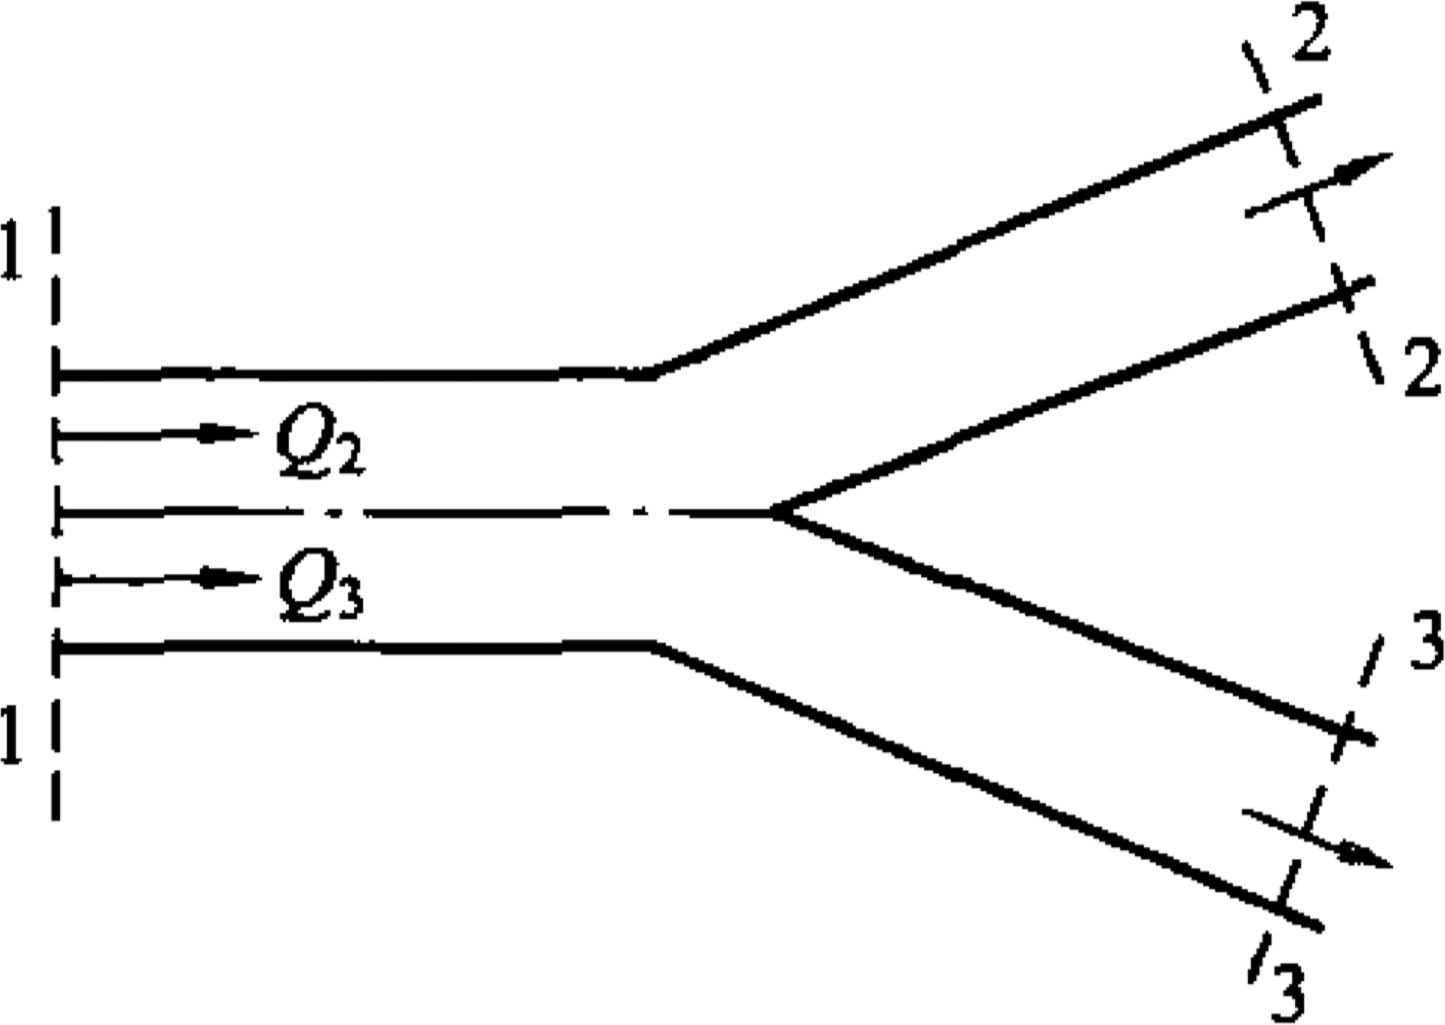
\includegraphics[width=\linewidth,height=0.45\textheight,keepaspectratio]{slides_assets/fluid_deck04/branch-Y.png}\\
      {\scriptsize 图：源讲义原图}
  \end{columns}
  \TLtakeaway{分岔连续性不是新定律，只是把一个出流断面换成多个出流断面。}
\end{frame}

\begin{frame}{算例 C-1：串联三段管求流速}
  已知串联管道流量 $Q=0.05\,\mathrm{m^3/s}$，三段直径分别为 $d_1=20\,\mathrm{cm}$、$d_2=15\,\mathrm{cm}$、$d_3=10\,\mathrm{cm}$。求各段平均流速。
  \begin{center}
  \begin{tikzpicture}[scale=0.64,>={Stealth[length=5pt]}]
    \draw[TLprimary,line width=13pt,line cap=butt] (-3,0)--(-1,0);
    \draw[TLprimary,line width=10pt,line cap=butt] (-1,0)--(1,0);
    \draw[TLprimary,line width=7pt,line cap=butt] (1,0)--(3,0);
    \draw[white,line width=6pt,line cap=butt] (-3,0)--(-1,0);
    \draw[white,line width=4pt,line cap=butt] (-1,0)--(1,0);
    \draw[white,line width=2.7pt,line cap=butt] (1,0)--(3,0);
    \draw[->,TLaccent,thick] (-3.4,0)--(-2.5,0) node[midway,above] {$Q$};
    \node[TLinkSoft] at (-2,-0.75) {$d_1=20\,\mathrm{cm}$};
    \node[TLinkSoft] at (0,-0.75) {$d_2=15\,\mathrm{cm}$};
    \node[TLinkSoft] at (2,-0.75) {$d_3=10\,\mathrm{cm}$};
  \end{tikzpicture}
  \end{center}
  \[
    A_1=\pi(0.1)^2=0.03142\,\mathrm{m^2},\quad
    v_1=\frac{0.05}{0.03142}\approx1.59\,\mathrm{m/s}.
  \]
  \[
    A_2=\pi(0.075)^2=0.01767\,\mathrm{m^2},\quad
    v_2=\frac{0.05}{0.01767}\approx2.83\,\mathrm{m/s}.
  \]
  \TLtakeaway{同一个 $Q$ 穿过不同管径时，速度只由 $v=Q/A$ 决定。}
\end{frame}

\begin{frame}{算例 C-1 续：最细管段}
  继续使用 $Q=0.05\,\mathrm{m^3/s}$，最细管段直径 $d_3=10\,\mathrm{cm}$，半径为 $0.05\,\mathrm m$。
  \[
    A_3=\pi(0.05)^2=0.007854\,\mathrm{m^2}.
  \]
  \[
    v_3=\frac{Q}{A_3}
    =
    \frac{0.05}{0.007854}
    \approx6.37\,\mathrm{m/s}.
  \]
  \begin{center}
  \vspace{2pt}
  \small
  \begin{tabular}{@{}lrrr@{}}
    \toprule
    管段 & $A\,(\mathrm{m^2})$ & $Q\,(\mathrm{m^3/s})$ & $v\,(\mathrm{m/s})$ \\
    \midrule
    1 & 0.03142 & 0.05 & 1.59 \\
    2 & 0.01767 & 0.05 & 2.83 \\
    3 & 0.007854 & 0.05 & 6.37 \\
    \bottomrule
  \end{tabular}
  \end{center}
  \TLtakeaway{面积约缩小到四分之一时，平均流速约增大到四倍；这就是连续性的数量级直觉。}
\end{frame}

\begin{frame}{算例 C-2：分岔管流量分配}
  总管流量 $Q_{\mathrm{main}}=0.1\,\mathrm{m^3/s}$，分到支路 1 和支路 2。支路 1 直径 $10\,\mathrm{cm}$，速度 $v_1=3\,\mathrm{m/s}$；支路 2 直径 $8\,\mathrm{cm}$。求 $Q_2$ 与 $v_2$。
  \[
    A_1=\pi(0.05)^2=0.007854\,\mathrm{m^2},\quad
    Q_1=v_1A_1=3\times0.007854=0.02356\,\mathrm{m^3/s}.
  \]
  \[
    Q_2=Q_{\mathrm{main}}-Q_1=0.1-0.02356=0.07644\,\mathrm{m^3/s}.
  \]
  支路 2 面积为 $A_2=\pi(0.04)^2=0.005027\,\mathrm{m^2}$，所以
  \[
    v_2=\frac{0.07644}{0.005027}\approx15.21\,\mathrm{m/s}.
  \]
  \TLtakeaway{分岔题先用已知支路速度算该支路流量，再用总流量守恒求未知支路。}
\end{frame}

% =============================================================================
% D. 4.4.2 恒定总流的动量方程
% =============================================================================
\TLsection{4.4.2 恒定总流的动量方程}

\begin{frame}{起点：控制体动量积分形式}
  目标：把动量积分形式应用到两过水断面控制体。本帧先写完整式子，再列出恒定总流的简化条件。\proofskipnote
  \[
    \frac{\partial}{\partial t}\iiint_V\rho\vc u\,\rd V
    +
    \iint_S\rho\vc u(\vc u\cdot\vc n)\,\rd A
    =
    \vc F_{\mathrm{body}}+\vc F_{\mathrm{surface}}.
  \]
  对恒定总流：
  \begin{itemize}
    \item 时间项为零；
    \item 侧壁没有穿透流量；
    \item $S_1,S_2$ 取过水断面，使 $\vc u$ 与断面法线共线；
    \item 合外力记为 $\sum\vc F$。
  \end{itemize}
  \TLtakeaway{动量方程的左边不是速度差，而是“流出带走的动量流量减去流入带来的动量流量”。}
\end{frame}

\begin{frame}{动量流量差：得到 (T4)}
  进度：上一帧消去了非断面通量。本帧先写某一坐标方向 $s$ 的标量分量，再合成矢量式。\proofskipnote
  若断面不均匀性暂时用 $\beta_i$ 表示，则 $s$ 方向动量方程为
  \[
    \sum F_s
    =
    \rho Q\left(\beta_2 v_{2s}-\beta_1 v_{1s}\right). \tag{T4}
  \]
  合成矢量写法为
  \[
    \sum\vc F
    =
    \rho Q\left(\beta_2\vc v_2-\beta_1\vc v_1\right).
  \]
  \begin{itemize}
    \item $Q$ 恒取正值，不带方向。
    \item 方向信息放在速度分量 $v_{is}$ 或速度矢量 $\vc v_i$ 中。
  \end{itemize}
  \TLtakeaway{入口项前的负号已经在“出口减入口”中体现，列分量式时不要再额外重复加负号。}
\end{frame}

\begin{frame}{动量修正系数 $\beta$：定义与不等式}
  断面速度不均匀时，不能把动量流量简单写成 $\rho Q\vc v$。需要\TLterm{动量修正系数} $\beta$ 修正。\proofskipnote
  \[
    \boxed{\beta=\frac{1}{A}\iint_A\left(\frac{u}{v}\right)^2\rd A\ge1.} \tag{T5}
  \]
  其中 $v=A^{-1}\iint_Au\,\rd A$。由 Cauchy--Schwarz 不等式：
  \[
    \left(\iint_Au\,\rd A\right)^2
    \le
    \left(\iint_Au^2\,\rd A\right)\left(\iint_A1^2\,\rd A\right).
  \]
  因为 $\iint_A1^2\rd A=A$，整理后正好得到 $\beta\ge1$。
  \TLtakeaway{$\beta$ 衡量断面速度分布的不均匀程度；越不均匀，同样平均速度携带的动量流量越大。}
\end{frame}

\begin{frame}{动量修正系数的典型取值}
  \begin{columns}[T]
    \column{0.46\textwidth}
      \begin{center}
      \small
      \begin{tabular}{@{}ll@{}}
        \toprule
        速度分布 & $\beta$ \\
        \midrule
        完全均匀 & $1$ \\
        圆管层流 & $4/3\approx1.33$ \\
        紊流 & $1.02$--$1.05$ \\
        工程近似 & 常取 $1$ \\
        \bottomrule
      \end{tabular}
      \end{center}
    \column{0.54\textwidth}
      \centering
      \begin{tikzpicture}[scale=0.72,>={Stealth[length=5pt]}]
        \draw[TLprimaryDark,thick] (-2.3,-0.7)--(-2.3,0.8);
        \draw[TLprimaryDark,thick] (-2.3,-0.7)--(-0.4,-0.7);
        \draw[TLaccent,thick,domain=-0.7:0.7,samples=40] plot ({-2.3+1.5*(1-\x*\x/0.49)}, {\x});
        \node[TLinkSoft] at (-1.35,-1.1) {层流抛物线};
        \draw[TLprimaryDark,thick] (0.6,-0.7)--(0.6,0.8);
        \draw[TLprimaryDark,thick] (0.6,-0.7)--(2.5,-0.7);
        \draw[TLaccent,thick] (0.6,-0.6) .. controls (2.0,-0.4) and (2.25,0.4) .. (0.8,0.65);
        \node[TLinkSoft] at (1.55,-1.1) {紊流更平坦};
      \end{tikzpicture}
  \end{columns}
  \TLtakeaway{多数工程水流是紊流，$\beta$ 接近 $1$；但写公式时保留 $\beta$ 能提醒我们断面速度分布被平均过。}
\end{frame}

\begin{frame}{恒定总流动量方程：矢量形式 (T6)}
  对不可压缩液体，密度 $\rho$ 视为常数。两断面无分岔时，恒定总流动量方程为
  \[
    \boxed{\sum\vc F=\rho Q\left(\beta_2\vc v_2-\beta_1\vc v_1\right).} \tag{T6}
  \]
  这是矢量方程，实际计算通常分解为坐标分量：
  \[
    \sum F_x=\rho Q\left(\beta_2v_{2x}-\beta_1v_{1x}\right),\quad
    \sum F_y=\rho Q\left(\beta_2v_{2y}-\beta_1v_{1y}\right).
  \]
  \begin{itemize}
    \item $\sum\vc F$ 是外界对控制体内流体的合力。
    \item 若题目要流体对固体的力，最后还要取反。
  \end{itemize}
  \TLtakeaway{动量方程能正交分解；这与后续能量方程的标量性质不同。}
\end{frame}

\begin{frame}{分岔总流的动量方程}
  分岔时，对每个出口加上动量流量，对每个入口减去动量流量。
  \[
    \sum\vc F
    =
    \rho\left(
      Q_2\beta_2\vc v_2
      +Q_3\beta_3\vc v_3
      -Q_1\beta_1\vc v_1
    \right).
  \]
  \begin{columns}[T]
    \column{0.5\textwidth}
      \begin{itemize}
        \item 每个 $Q_i$ 仍恒取正值。
        \item 每个 $\vc v_i$ 按坐标轴方向分量定号。
        \item 入流项的负号来自公式结构。
      \end{itemize}
    \column{0.5\textwidth}
      \centering
      \begin{tikzpicture}[scale=0.68,>={Stealth[length=5pt]}]
        \draw[TLprimary,line width=8pt,line cap=round] (-2,0)--(-0.4,0);
        \draw[TLprimary,line width=8pt,line cap=round] (-0.4,0)--(1.6,0.8);
        \draw[TLprimary,line width=8pt,line cap=round] (-0.4,0)--(1.6,-0.8);
        \draw[white,line width=4pt,line cap=round] (-2,0)--(-0.4,0)--(1.6,0.8);
        \draw[white,line width=4pt,line cap=round] (-0.4,0)--(1.6,-0.8);
        \draw[->,TLaccent,thick] (-1.7,0)--(-0.9,0) node[midway,above] {$\vc v_1$};
        \draw[->,TLaccent,thick] (0.15,0.22)--(1.0,0.56) node[midway,above] {$\vc v_2$};
        \draw[->,TLaccent,thick] (0.15,-0.22)--(1.0,-0.56) node[midway,below] {$\vc v_3$};
      \end{tikzpicture}
  \end{columns}
  \TLtakeaway{多出口问题没有新符号规则；只是把“出口总和减入口总和”逐支路写出来。}
\end{frame}

\begin{frame}{解题要点：控制体、受力、坐标}
  动量方程题本质上是控制体版本的牛顿第二定律。不要先代公式，要先画研究对象。
  \begin{columns}[T]
    \column{0.56\textwidth}
      \begin{enumerate}
        \item 画\TLterm{控制体图}，标出入流和出流断面。
        \item 做\TLterm{受力分析}：重力 $W$、断面压力 $p_1A_1,p_2A_2$、侧壁对流体的力 $R$。
        \item 选坐标系，尽量让速度方向投影简单。
        \item 沿每个坐标轴列分量动量方程。
        \item 用\TLterm{牛顿第三定律}把流体受力换成固体受力。
      \end{enumerate}
    \column{0.44\textwidth}
      \centering
      \begin{tikzpicture}[scale=0.66,>={Stealth[length=5pt]}]
        \draw[fill=TLprimaryTint,draw=TLprimary,thick] (-1.8,-0.75) rectangle (1.8,0.75);
        \draw[->,TLaccent,thick] (-2.45,0)--(-1.8,0) node[midway,above] {$p_1A_1$};
        \draw[->,TLaccent,thick] (2.45,0)--(1.8,0) node[midway,above] {$p_2A_2$};
        \draw[->,TLprimaryDark,thick] (0,1.25)--(0,0.75) node[midway,right] {$R$};
        \draw[->,TLinkSoft,thick] (0,-0.1)--(0,-1.1) node[below] {$W$};
        \draw[->,TLprimaryDark,thick] (-2.1,-1.35)--(-1.25,-1.35) node[right] {$x$};
      \end{tikzpicture}
  \end{columns}
  \TLtakeaway{未知的壁面对流体作用力先记为 $R$；题目若问流体对固体的力，答案是 $-R$。}
\end{frame}

\begin{frame}{解题要点：正负号三规则}
  动量方程最常见错误是方向符号错。下面三条规则要同时使用。
  \begin{center}
  \vspace{3pt}
  \small
  \begin{tabular}{@{}ll@{}}
    \toprule
    规则 & 含义 \\
    \midrule
    $Q$ 恒正 & 体积流量只表示每秒通过多少体积，不带坐标方向 \\
    速度分量定号 & $v_x,v_y$ 按坐标轴正方向为正，反方向为负 \\
    入流项已带负号 & 公式已经是“出口动量流量减入口动量流量” \\
    \bottomrule
  \end{tabular}
  \end{center}
  \[
    \sum F_x
    =
    \rho\left(\sum_{\text{出口}}Q\beta v_x-\sum_{\text{入口}}Q\beta v_x\right).
  \]
  \TLtakeaway{不要把入流速度分量先取负、又在入口项前再取负；这样会把入口动量方向翻错。}
\end{frame}

\begin{frame}{算例 D-1：射流冲击固定平板}
  水平水射流垂直冲击固定平板，射流直径 $d=5\,\mathrm{cm}$，入口速度 $v_1=10\,\mathrm{m/s}$。水沿平板切向散开，求水对平板的力。
  \begin{columns}[T]
    \column{0.5\textwidth}
      \begin{itemize}
        \item 控制体：喷口出口到平板前的水团和薄膜。
        \item 取 $x$ 轴沿射流方向。
        \item 入口 $v_{1x}=10\,\mathrm{m/s}$。
        \item 出口沿平板切向散开，合 $x$ 分量为 $v_{2x}=0$。
        \item 取 $\beta=1$，各处相对压强为零。
      \end{itemize}
    \column{0.5\textwidth}
      \centering
      \begin{tikzpicture}[scale=0.68,>={Stealth[length=5pt]}]
        \draw[TLprimary,line width=8pt] (-2.4,0)--(-0.5,0);
        \draw[->,TLaccent,thick] (-2.2,0.3)--(-1.1,0.3) node[midway,above] {$v_1$};
        \draw[TLprimaryDark,line width=3pt] (-0.25,-1.1)--(-0.25,1.1);
        \draw[->,TLprimary,thick] (-0.25,0.1).. controls (0.25,0.6) and (0.75,0.85)..(1.3,0.95);
        \draw[->,TLprimary,thick] (-0.25,-0.1).. controls (0.25,-0.6) and (0.75,-0.85)..(1.3,-0.95);
        \node[TLinkSoft] at (0.25,-1.45) {出口切向，$x$ 分量为零};
      \end{tikzpicture}
  \end{columns}
  \TLtakeaway{平板把射流的 $x$ 向动量降为零；这个动量损失对应平板受力。}
\end{frame}

\begin{frame}{算例 D-1 计算：平板受力}
  断面面积和流量为
  \[
    A=\pi(0.025)^2=0.001963\,\mathrm{m^2},\qquad
    Q=v_1A=10\times0.001963=0.01963\,\mathrm{m^3/s}.
  \]
  对流体列 $x$ 方向动量方程：
  \[
    \sum F_x
    =
    \rho Q(v_{2x}-v_{1x})
    =
    1000\times0.01963\times(0-10)
    =
    -196.3\,\mathrm N.
  \]
  这表示平板对流体的力沿 $-x$ 方向。由牛顿第三定律，流体对平板的力为
  \[
    \boxed{196.3\,\mathrm N\quad \text{沿 }+x\text{ 方向}.}
  \]
  \TLtakeaway{动量方程先给“外界对流体”的合力；求“流体对平板”必须反向。}
\end{frame}

\begin{frame}{算例 D-2：分叉管镇墩的控制体}
  管道直径 $d_1=0.3\,\mathrm m$，入口压强 $p_1=150\,\mathrm{kPa}$ 表压，入口流量 $Q_1=0.2\,\mathrm{m^3/s}$。两支路等分流量，$Q_2=Q_3=0.1\,\mathrm{m^3/s}$，出口直径均为 $0.2\,\mathrm m$，夹角为 $\pm30^\circ$。
  \begin{center}
  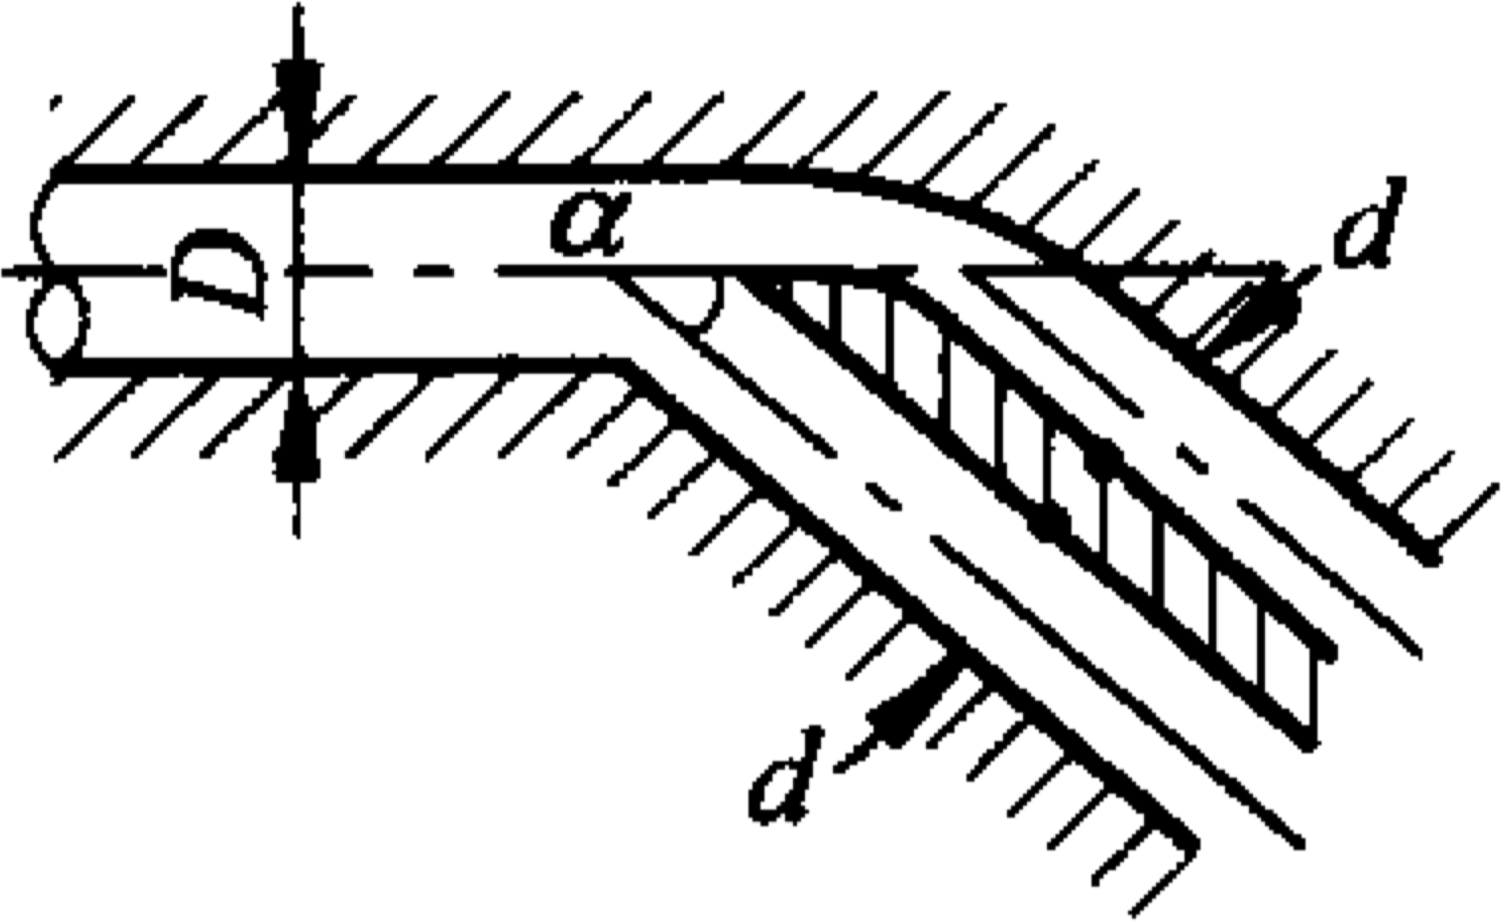
\includegraphics[width=0.72\textwidth,height=0.48\textheight,keepaspectratio]{slides_assets/fluid_deck04/ex-anchor-branch.png}\\
  {\scriptsize 图：源讲义原图}
  \end{center}
  \TLtakeaway{对称分叉让 $y$ 方向动量和压力贡献相互抵消，主要未知是 $x$ 方向镇墩受力。}
\end{frame}

\begin{frame}{算例 D-2 计算（一）：速度与动量流量}
  入口面积和速度为
  \[
    A_1=\pi(0.15)^2=0.07069\,\mathrm{m^2},\qquad
    v_1=\frac{0.2}{0.07069}\approx2.83\,\mathrm{m/s}.
  \]
  支路面积和速度为
  \[
    A_2=A_3=\pi(0.1)^2=0.03142\,\mathrm{m^2},\qquad
    v_2=v_3=\frac{0.1}{0.03142}\approx3.18\,\mathrm{m/s}.
  \]
  出口动量流量的 $x$ 分量减入口动量流量：
  \[
    1000\left(0.1\times3.18\times0.866\times2-0.2\times2.83\right)
    =
    1000(-0.0152)\approx-15.2\,\mathrm N.
  \]
  \TLtakeaway{动量流量的净 $x$ 变化很小；本题的主要水平力来自入口压力。}
\end{frame}

\begin{frame}{算例 D-2 计算（二）：压力项与镇墩受力}
  取出口为大气表压零。设管壁对流体的水平合力为 $R_x$，则
  \[
    p_1A_1+R_x
    =
    \rho(Q_2v_2\cos30^\circ+Q_3v_3\cos30^\circ-Q_1v_1).
  \]
  压力项为
  \[
    p_1A_1=150000\times0.07069=10604\,\mathrm N.
  \]
  所以
  \[
    R_x=-15.2-10604=-10619.2\,\mathrm N.
  \]
  这是管壁对流体的力，沿 $-x$。因此流体对管道和镇墩的力为
  \[
    \boxed{10619.2\,\mathrm N\quad \text{沿 }+x\text{ 方向}.}
  \]
  对称性给出 $y$ 方向合力为零。
  \TLtakeaway{镇墩题必须把压力力和动量流量同时放进方程；只看动量流量会低估很多。}
\end{frame}

\begin{frame}{算例 D-3a：底坎过流的已知量与目标}
  渠道为矩形明渠，宽度 $b=1.0\,\mathrm m$。上游为缓流，水深 $h_1=2.0\,\mathrm m$，平均速度 $v_1=1.0\,\mathrm{m/s}$；底坎抬高 $\Delta z=0.10\,\mathrm m$，忽略能量损失。
  \begin{columns}[T]
    \column{0.48\textwidth}
      \begin{center}
      \footnotesize
      \setlength{\tabcolsep}{4pt}
      \begin{tabular}{@{}ll@{}}
        \toprule
        已知量 & 数值 \\
        \midrule
        单宽流量 & $q=v_1h_1=1.0\times2.0=2.0\,\mathrm{m^2/s}$ \\
        密度 & $\rho=1000\,\mathrm{kg/m^3}$ \\
        重力加速度 & $g=9.81\,\mathrm{m/s^2}$ \\
        水平宽度 & $b=1.0\,\mathrm m$ \\
        \bottomrule
      \end{tabular}
      \end{center}
      目标是先由连续性与无损能量方程求 $h_2,v_2$，再用水平动量方程求底坎对水流的反力大小 $R$。
    \column{0.52\textwidth}
      \centering
      \begin{tikzpicture}[scale=0.70,>={Stealth[length=5pt]}]
        \fill[TLprimaryTint] (-3,0) -- (-0.7,0) -- (-0.1,0.28) -- (0.8,0.28) -- (1.4,0) -- (3,0) -- (3,1.25) -- (-3,1.45) -- cycle;
        \draw[TLprimary,thick] (-3,0)--(-0.7,0)--(-0.1,0.28)--(0.8,0.28)--(1.4,0)--(3,0);
        \draw[TLprimaryDark,thick] (-3,1.45)--(3,1.25);
        \draw[->,TLaccent,thick] (-2.65,0.65)--(-1.65,0.65) node[midway,above] {$v_1$};
        \draw[->,TLaccent,thick] (1.55,0.62)--(2.45,0.62) node[midway,above] {$v_2$};
        \draw[<->,TLprimaryDark,thick] (-2.65,0)--(-2.65,1.42) node[midway,left] {$h_1$};
        \draw[<->,TLprimaryDark,thick] (2.55,0)--(2.55,1.25) node[midway,right] {$h_2$};
        \draw[<->,TLinkSoft,thick] (0.35,0)--(0.35,0.28) node[midway,right] {$\Delta z$};
        \node[TLinkSoft] at (0,-0.42) {单位宽度计算；本题 $b=1.0\,\mathrm m$};
      \end{tikzpicture}
  \end{columns}
  \TLtakeaway{底坎题不能先假定下游水深；必须先用能量方程求出与给定流量自洽的 $h_2$。}
\end{frame}

\begin{frame}{算例 D-3b：连续性与无损能量求 $h_2$}
  进度：上一帧确定 $q=2.0\,\mathrm{m^2/s}$。本帧先求真实下游水深，再选与缓流相容的根。
  \begin{columns}[T]
    \column{0.62\textwidth}
      \footnotesize
      \[
        v_2=\frac{q}{h_2}=\frac{2.0}{h_2}.
      \]
      \[
        h_1+\frac{v_1^2}{2g}
        =
        h_2+\Delta z+\frac{v_2^2}{2g}. \tag{T7}
      \]
      \[
        2.0+\frac{1.0^2}{2\times9.81}
        =
        h_2+0.10+\frac{(2.0/h_2)^2}{2\times9.81}.
      \]
      \[
        2.050968
        =
        h_2+0.10+\frac{4.0}{19.62h_2^2}.
      \]
      \[
        1.950968=h_2+\frac{0.203874}{h_2^2}.
      \]
    \column{0.38\textwidth}
      \footnotesize
      两边乘以 $h_2^2$：
      \[
        h_2^3-1.950968h_2^2+0.203874=0.
      \]
      正实根为
      \[
        h_2=0.358\,\mathrm m,\qquad h_2=1.894\,\mathrm m.
      \]
      对较大根：
      \[
        Fr_2=\frac{1.056}{\sqrt{9.81\times1.894}}\approx0.245<1.
      \]
      根的选择：小根对应急流，较大根对应亚临界缓流。题设无水跃、无损失，所以保留
      \[
        \boxed{h_2=1.894\,\mathrm m.}
      \]
  \end{columns}
\end{frame}

\begin{frame}{算例 D-3c：水平动量方程求底坎反力}
  进度：上一帧得到 $h_2=1.894143979\,\mathrm m$。本帧把静水压力差与动量通量差放进同一个水平动量方程。
  \[
    v_2=\frac{2.0}{1.894143979}=1.055886\,\mathrm{m/s}.
  \]
  压力合力差为
  \[
    \frac12\rho gb(h_1^2-h_2^2)
    =
    0.5\times1000\times9.81\times(2.0^2-1.894143979^2).
  \]
  \[
    =
    4905\times(4.000000-3.587781)
    =
    2021.93\,\mathrm{N/m}.
  \]
  动量通量增加量为
  \[
    \rho qb(v_2-v_1)
    =
    1000\times2.0\times1.0\times(1.055886-1.0)
    =
    111.77\,\mathrm{N/m}.
  \]
  \[
    \boxed{R=2021.93-111.77=1910.16\,\mathrm{N/m}.}
  \]
  \TLtakeaway{$R>0$ 表示底坎必须给水流一个向上游的水平作用；水流对底坎的水平作用大小相同、方向向下游。}
\end{frame}

\begin{frame}{算例 D-3d：为什么 $R$ 为正}
  上游水深略大于下游水深，所以上游静水压力三角形更大；同时水流只从 $1.000$ 加速到 $1.056\,\mathrm{m/s}$，所需动量增量很小。
  \begin{center}
  \begin{tikzpicture}[scale=0.75,>={Stealth[length=5pt]}]
    \fill[TLprimaryTint] (-3,0) -- (-0.7,0) -- (-0.1,0.28) -- (0.8,0.28) -- (1.4,0) -- (3,0) -- (3,1.22) -- (-3,1.42) -- cycle;
    \draw[TLprimary,thick] (-3,0)--(-0.7,0)--(-0.1,0.28)--(0.8,0.28)--(1.4,0)--(3,0);
    \draw[TLprimaryDark,thick] (-3,1.42)--(3,1.22);
    \draw[fill=TLaccentLight,draw=TLaccent,thick] (-3.35,0)--(-3.35,1.42)--(-2.82,0)--cycle;
    \draw[fill=TLaccentLight,draw=TLaccent,thick] (3.35,0)--(3.35,1.22)--(2.90,0)--cycle;
    \node[TLaccent,align=center,font=\small] at (-2.55,1.62) {上游压力\\$2021.93$ 的主来源};
    \node[TLaccent,align=center,font=\small] at (2.55,1.42) {下游压力\\略小};
    \draw[->,TLprimaryDark,thick] (0.60,0.62)--(-0.35,0.62) node[midway,above] {$R$};
    \draw[->,TLinkSoft,thick] (1.25,0.42)--(2.10,0.42) node[midway,below] {$v_2-v_1$ 小};
    \node[TLinkSoft,align=center,text width=9.5cm] at (0,-0.55)
      {水平动量平衡：压力差向下游很大，实际动量增量很小，差额由底坎向上游的反力平衡。};
  \end{tikzpicture}
  \end{center}
  \TLtakeaway{这类底坎题的方向判断靠两项比较：静水压力差推动水向下游，底坎反力抵消多余的推动。}
\end{frame}

% =============================================================================
% E. 4.4.3 恒定元流的能量方程（伯努利方程）
% =============================================================================
\TLsection{4.4.3 恒定元流的能量方程（伯努利方程）}

\begin{frame}{从静水压强桥接到运动流体}
  水静力学给过一个非常简单的守恒量：静止、不可压、只受重力时，任意两点满足
  \[
    z+\frac{p}{\rho g}=\text{常数}.
  \]
  现在流体开始运动，动能不能再忽略。本节的问题是：\TLterm{沿同一条流线运动的流体微团，有没有“势能 + 动能”的守恒量？}
  \begin{center}
  \begin{tikzpicture}[scale=0.72,>={Stealth[length=5pt]}]
    \node[draw=TLprimary,fill=TLprimaryTint,rounded corners=2pt,minimum width=3.1cm,minimum height=0.7cm] (hydro) at (-3.2,0) {静止：$z+p/(\rho g)$};
    \node[draw=TLaccent,fill=TLaccentLight,rounded corners=2pt,minimum width=3.2cm,minimum height=0.7cm] (move) at (1.0,0) {运动：再加 $u^2/(2g)$};
    \node[draw=TLprimaryDark,fill=white,rounded corners=2pt,minimum width=3.2cm,minimum height=0.7cm] (road) at (5.0,0) {沿流线积分欧拉方程};
    \draw[->,TLprimaryDark,thick] (hydro)--(move);
    \draw[->,TLprimaryDark,thick] (move)--(road);
  \end{tikzpicture}
  \end{center}
  \TLtakeaway{伯努利方程不是孤立公式；它是水静力学“测压管水头守恒”加入动能后的运动版本。}
\end{frame}

\begin{frame}{沿流线推导伯努利方程}
  进度：本帧从理想流体的欧拉方程出发，只沿同一条流线做积分。\proofskipnote
  对恒定、无粘、不可压流体，欧拉方程写成
  \[
    \rho\DDt{\vc u}=-\grad p+\rho\vc g.
  \]
  沿流线取微小位移 $\rd\vc s$。速度方向与 $\rd\vc s$ 相同，且 $z$ 轴向上，所以
  \[
    \rho\DDt{\vc u}\cdot\rd\vc s
    =
    -\grad p\cdot\rd\vc s+\rho\vc g\cdot\rd\vc s.
  \]
  \[
    \rho u\,\rd u=-\rd p-\rho g\,\rd z.
  \]
  \[
    \frac{u\,\rd u}{g}=-\frac{\rd p}{\rho g}-\rd z.
  \]
  \[
    \rd z+\frac{\rd p}{\rho g}+\frac{u\,\rd u}{g}=0.
  \]
  \[
    z+\frac{p}{\rho g}+\frac{u^2}{2g}=C.
  \]
\end{frame}

\begin{frame}{伯努利方程：三种水头的含义}
  在同一条流线上取点 1 和点 2，上一帧的常数 $C$ 在两点相同，因此
  \[
    \boxed{
    z_1+\frac{p_1}{\rho g}+\frac{u_1^2}{2g}
    =
    z_2+\frac{p_2}{\rho g}+\frac{u_2^2}{2g}.} \tag{T8}
  \]
  \begin{center}
  \footnotesize
  \setlength{\tabcolsep}{5pt}
  \begin{tabular}{@{}lll@{}}
    \toprule
    项 & 名称 & 物理意义 \\
    \midrule
    $z$ & 位置水头 & 单位重量流体的重力势能 \\
    $p/(\rho g)$ & 压强水头 & 单位重量流体的压强势能 \\
    $u^2/(2g)$ & 流速水头 & 单位重量流体的动能 \\
    \bottomrule
  \end{tabular}
  \end{center}
  \[
    \text{测压管水头}=z+\frac{p}{\rho g},\qquad
    H=z+\frac{p}{\rho g}+\frac{u^2}{2g}.
  \]
  \TLtakeaway{伯努利方程说的是同一流线上总水头 $H$ 守恒；不同流线的常数一般不同。}
\end{frame}

\begin{frame}{伯努利方程的五个成立条件}
  伯努利方程强大，但条件也很严格。每个条件都对应推导中的一步。
  \begin{columns}[T]
    \column{0.52\textwidth}
      \small
      \begin{enumerate}
        \item 质量力只有重力：这样体力功才能写成 $-\rho g\,\rd z$。
        \item 恒定流：流线可看成流体微团的运动轨迹。
        \item 不可压缩：$\rho$ 为常数，$\rd p/(\rho g)$ 才能直接积分。
      \end{enumerate}
    \column{0.48\textwidth}
      \small
      \begin{enumerate}
        \setcounter{enumi}{3}
        \item 无粘理想流体：没有粘性耗散，机械能不转化为内能。
        \item 沿同一流线：常数 $C$ 是沿流线得到的，不是全流场同一个数。
      \end{enumerate}
      \TLwarnblock{实际流体}{
        实际水流有粘性，机械能会损失；此时要在方程右侧加水头损失 $h_w'$。
      }
  \end{columns}
\end{frame}

\begin{frame}{实际元流：加入水头损失 $h_w'$}
  若沿同一流线从点 1 到点 2 有粘性耗散，则点 1 的机械能不可能全部到达点 2。
  \[
    z_1+\frac{p_1}{\rho g}+\frac{u_1^2}{2g}
    =
    z_2+\frac{p_2}{\rho g}+\frac{u_2^2}{2g}
    +h_w'.
  \]
  \begin{columns}[T]
    \column{0.55\textwidth}
      \begin{itemize}
        \item $h_w'>0$ 表示从点 1 到点 2 的单位重量机械能损失。
        \item 损失来自粘性摩擦，把机械能转化为内能。
        \item 理想流体是 $h_w'=0$ 的特殊情况。
      \end{itemize}
    \column{0.45\textwidth}
      \centering
      \begin{tikzpicture}[scale=0.72,>={Stealth[length=5pt]}]
        \draw[TLprimary,line width=7pt,line cap=round] (-2.5,-0.35)--(2.5,-0.35);
        \draw[TLaccent,thick] (-2.4,1.1)--(2.4,0.35) node[right] {$H$};
        \draw[dashed,TLinkSoft,thick] (-2.4,1.1)--(2.4,1.1) node[right] {无损};
        \draw[<->,TLprimaryDark,thick] (1.6,0.45)--(1.6,1.05) node[midway,right] {$h_w'$};
        \node[TLinkSoft] at (0,-0.95) {总水头沿流动方向下降};
      \end{tikzpicture}
  \end{columns}
  \TLtakeaway{把 $h_w'$ 放在下游一侧，意思是：上游总水头 = 下游剩余总水头 + 中途损失。}
\end{frame}

\begin{frame}{应用 E-1：皮托管测流速}
  皮托管把迎流点处的流体“刹停”。停滞点速度为零，动能转化为压强升高。
  \begin{columns}[T]
    \column{0.57\textwidth}
      \small
      同一高度、忽略损失：
      \[
        z+\frac{p}{\rho g}+\frac{u^2}{2g}
        =
        z+\frac{p_0}{\rho g}+0.
      \]
      \[
        \frac{u^2}{2g}=\frac{p_0-p}{\rho g}.
      \]
      \[
        u^2=\frac{2(p_0-p)}{\rho}.
      \]
      \[
        \boxed{u=\sqrt{\frac{2(p_0-p)}{\rho}}.}
      \]
    \column{0.43\textwidth}
      \centering
      \begin{tikzpicture}[scale=0.68,>={Stealth[length=5pt]}]
        \draw[TLprimary,line width=8pt] (-2.6,0)--(1.2,0);
        \foreach \y in {-0.45,0,0.45}{
          \draw[->,TLaccent,thick] (-2.7,\y)--(-1.6,\y) node[midway,above] {$u$};
        }
        \draw[TLprimaryDark,line width=3pt] (0.5,-0.9)--(0.5,0.55)--(1.45,0.55);
        \draw[fill=TLaccentLight,draw=TLaccent,thick] (0.38,-0.05) circle (2pt);
        \node[TLinkSoft] at (1.35,0.88) {$p_0$};
        \node[TLinkSoft,align=center,text width=4.4cm] at (-0.25,-1.35) {停滞点：$u=0$，压强升为总压};
      \end{tikzpicture}
  \end{columns}
  \TLtakeaway{皮托管不是直接看速度，而是把速度水头转换成可测的压强差。}
\end{frame}

\begin{frame}{应用 E-2：文丘里管测流量}
  文丘里管用收缩段制造压强差，再由连续性和伯努利方程反推流量。
  \begin{columns}[T]
    \column{0.60\textwidth}
      \footnotesize
      连续性：
      \[
        A_1v_1=A_2v_2,\qquad v_2=\frac{A_1}{A_2}v_1.
      \]
      同高、无损：
      \[
        \frac{p_1}{\rho g}+\frac{v_1^2}{2g}
        =
        \frac{p_2}{\rho g}+\frac{v_2^2}{2g}.
      \]
      \[
        \frac{p_1-p_2}{\rho g}
        =
        \frac{\left[(A_1/A_2)^2-1\right]v_1^2}{2g}.
      \]
      \[
        v_1=
        \sqrt{\frac{2(p_1-p_2)}{\rho\left[(A_1/A_2)^2-1\right]}},
        \qquad Q=A_1v_1.
      \]
    \column{0.40\textwidth}
      \centering
      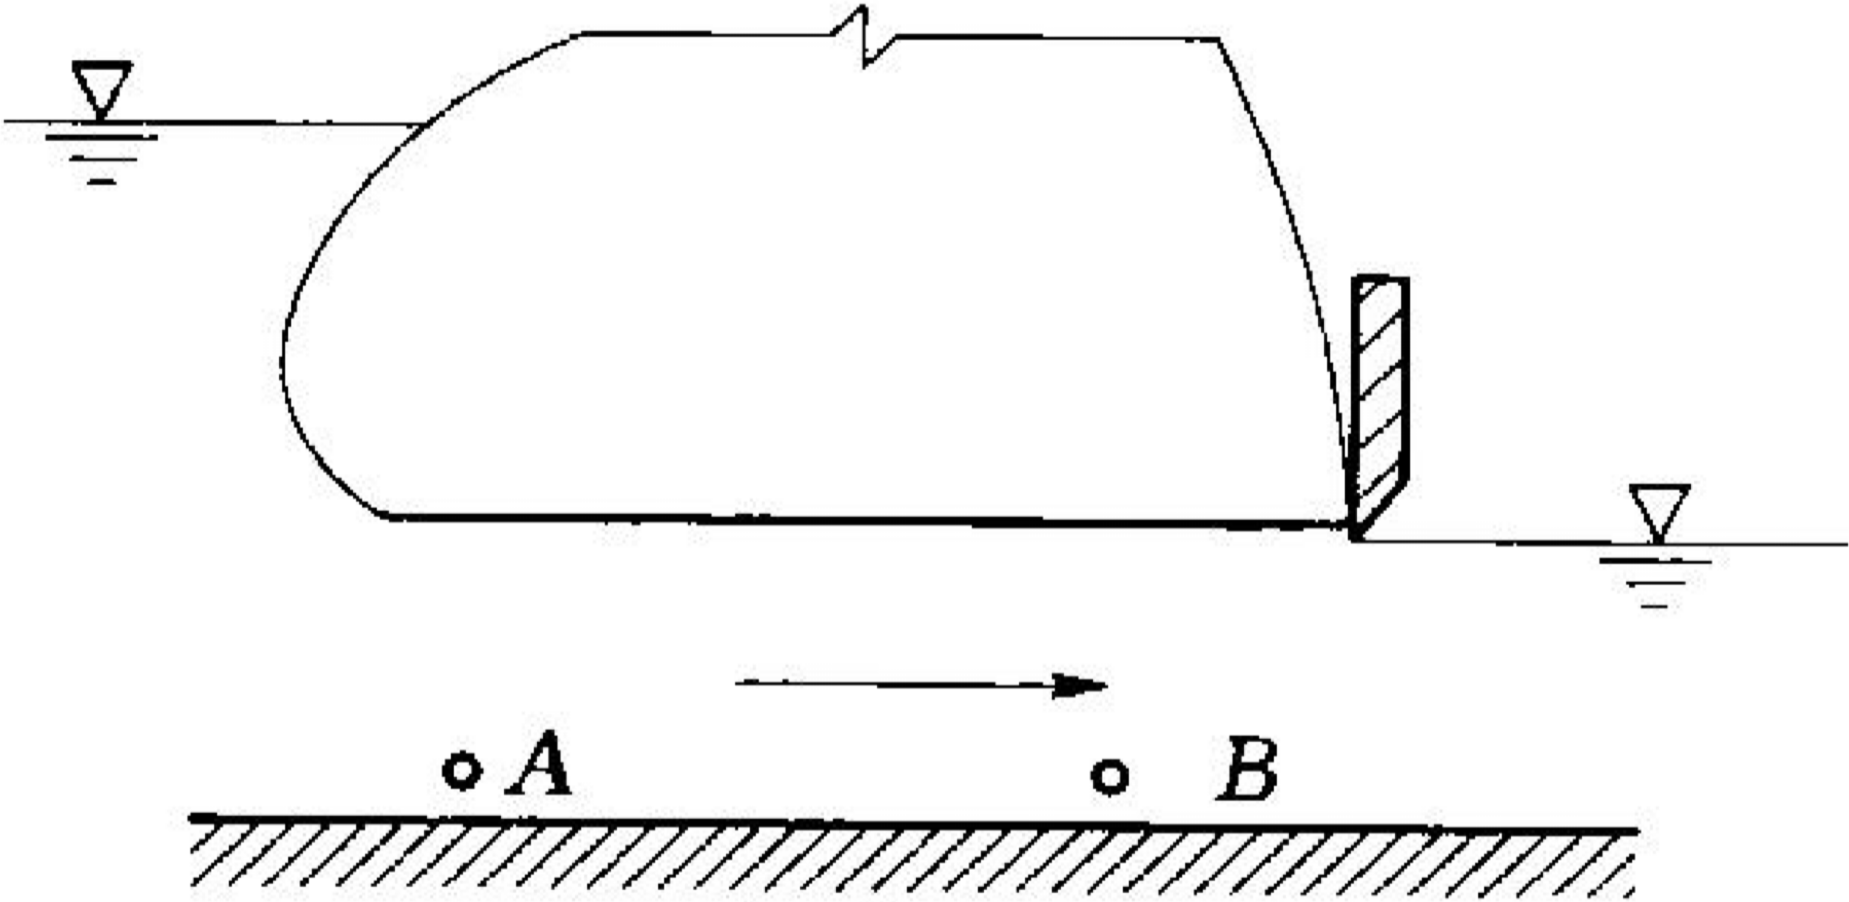
\includegraphics[width=\linewidth,height=0.45\textheight,keepaspectratio]{slides_assets/fluid_deck04/venturi.png}\\
      {\scriptsize 图：源讲义原图}
  \end{columns}
\end{frame}

\begin{frame}{水头线：把伯努利方程画出来}
  对理想流体，同一流线上的总水头线为水平线；测压管水头线随速度水头变化而升降。
  \begin{center}
  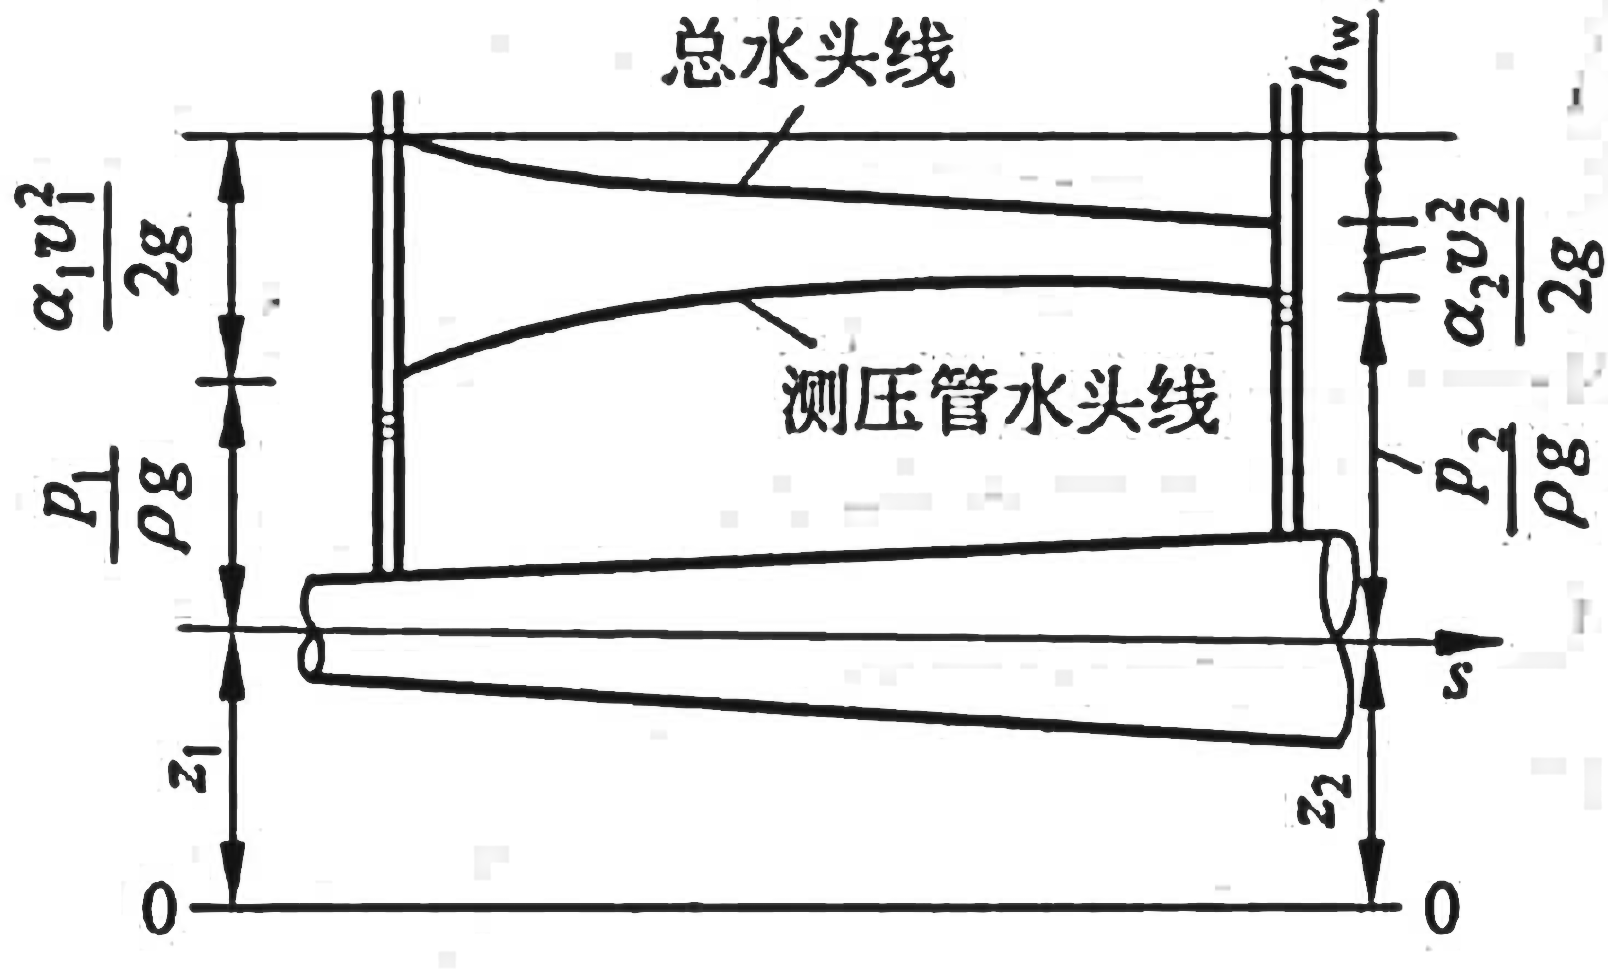
\includegraphics[width=0.72\textwidth,height=0.48\textheight,keepaspectratio]{slides_assets/fluid_deck04/head-lines.png}\\
  {\scriptsize 图：源讲义原图}
  \end{center}
  \TLtakeaway{总水头线到测压管水头线的竖向距离就是流速水头；这张图是伯努利方程的几何读法。}
\end{frame}

% =============================================================================
% F. 4.4.4 恒定总流的能量方程
% =============================================================================
\TLsection{4.4.4 恒定总流的能量方程}

\begin{frame}{从流线到过水断面：为什么要积分}
  伯努利方程只沿一条流线成立；真实管流和明渠流有有限过水断面，断面上速度通常不均匀。
  \begin{columns}[T]
    \column{0.58\textwidth}
      \small
      理想总流的能量流量写成
      \[
        \iint_A \rho gH\,u\,\rd A=\text{常数}.
      \]
      对均匀流或渐变流断面：
      \[
        z+\frac{p}{\rho g}\approx\text{断面常数}.
      \]
      速度项不能直接提出：
      \[
        \iint_A u^3\,\rd A\ne v^3A.
      \]
      因此总流能量方程需要\TLterm{动能修正系数}。
    \column{0.42\textwidth}
      \centering
      \begin{tikzpicture}[scale=0.70,>={Stealth[length=5pt]}]
        \draw[fill=TLprimaryTint,draw=TLprimary,thick] (0,0) ellipse (1.0 and 1.45);
        \foreach \y/\len in {-1.0/0.55,-0.55/1.05,0/1.35,0.55/1.05,1.0/0.55}{
          \draw[->,TLaccent,thick] (-0.25,\y)--++(\len,0);
        }
        \node[TLinkSoft,align=center,text width=4.2cm] at (0,-2.0) {断面速度分布不均匀，不能只用 $v^3A$ 代替};
      \end{tikzpicture}
  \end{columns}
\end{frame}

\begin{frame}{动能修正系数 $\alpha$}
  动能修正系数把真实速度分布携带的动能流量，折算成平均速度形式。
  \[
    \boxed{\alpha=\frac{1}{A}\iint_A\left(\frac{u}{v}\right)^3\rd A\ge1.}
  \]
  \begin{columns}[T]
    \column{0.54\textwidth}
      \footnotesize
      因为 $x^3$ 在 $x>0$ 上是凸函数，Jensen 不等式给出
      \[
        \frac1A\iint_A\left(\frac{u}{v}\right)^3\rd A
        \ge
        \left[\frac1A\iint_A\frac{u}{v}\rd A\right]^3=1.
      \]
      速度完全均匀时，处处 $u=v$，所以 $\alpha=1$。
    \column{0.46\textwidth}
      \footnotesize
      圆管层流 $u(r)=2v(1-r^2/R^2)$：
      \[
        \alpha=\frac1{\pi R^2}\int_0^R
        \left[2\left(1-\frac{r^2}{R^2}\right)\right]^3 2\pi r\,\rd r.
      \]
      令 $\xi=r^2/R^2$：
      \[
        \alpha=\int_0^1 8(1-\xi)^3\rd\xi=2.
      \]
      紊流常取 $\alpha\approx1.05$--$1.10$，工程近似常取 $1$。
  \end{columns}
\end{frame}

\begin{frame}{恒定总流能量方程}
  把断面能量流量写成平均水头形式，并加入实际水头损失，得到最常用的总流能量方程：
  \[
    \boxed{
    z_1+\frac{p_1}{\rho g}+\frac{\alpha_1v_1^2}{2g}
    =
    z_2+\frac{p_2}{\rho g}+\frac{\alpha_2v_2^2}{2g}+h_w.} \tag{T9}
  \]
  定义总流总水头
  \[
    H=z+\frac{p}{\rho g}+\frac{\alpha v^2}{2g},
  \]
  则
  \[
    H_1=H_2+h_w.
  \]
  水头损失按来源可写成
  \[
    h_w=\sum h_f+\sum h_j,
  \]
  其中 $h_f$ 是沿程损失，$h_j$ 是局部损失；具体计算留到后续水头损失章节。
  \TLtakeaway{总流能量方程是伯努利方程的断面平均版本；$\alpha$ 修正速度分布，$h_w$ 记录粘性损失。}
\end{frame}

\begin{frame}{动量方程与能量方程的关键区别}
  两个方程都来自守恒思想，但回答的问题不同。选错方程会让未知量变得很难求。
  \begin{center}
  \small
  \setlength{\tabcolsep}{5pt}
  \begin{tabular}{@{}lll@{}}
    \toprule
    对比项 & 动量方程 & 能量方程 \\
    \midrule
    类型 & 矢量方程，可分解 & 标量方程，不可分解 \\
    适用 & 求外力、冲量、支座反力 & 求水头、流速、压强 \\
    修正系数 & $\beta$，修正动量通量 & $\alpha$，修正动能通量 \\
    损失项 & 不直接出现 & $h_w$ 显式出现 \\
    典型图像 & 控制体受力图 & 总水头线与测压管水头线 \\
    \bottomrule
  \end{tabular}
  \end{center}
  \TLtakeaway{两方程互补：求力优先想动量方程，求压强、流速和水头优先想能量方程。}
\end{frame}

\begin{frame}{流体机械：水泵加水头，水轮机取水头}
  若两断面之间有流体机械，机械会对单位重量流体输入或取出机械能。
  \[
    z_1+\frac{p_1}{\rho g}+\frac{\alpha_1v_1^2}{2g}
    \pm h_m
    =
    z_2+\frac{p_2}{\rho g}+\frac{\alpha_2v_2^2}{2g}+h_w.
  \]
  \begin{columns}[T]
    \column{0.54\textwidth}
      \begin{itemize}
        \item 水泵：向水流输入机械能，用 $+h_m$。
        \item 水轮机：从水流取出机械能，用 $-h_m$。
        \item $h_m$ 的量纲是长度，表示单位重量流体增减的机械能。
      \end{itemize}
    \column{0.46\textwidth}
      \centering
      \begin{tikzpicture}[scale=0.70,>={Stealth[length=5pt]}]
        \draw[TLprimary,line width=7pt,line cap=round] (-2.7,0)--(-0.7,0);
        \draw[TLprimary,line width=7pt,line cap=round] (0.7,0)--(2.7,0);
        \draw[fill=TLaccentLight,draw=TLaccent,thick] (0,0) circle (0.62);
        \draw[->,TLaccent,thick] (-2.4,0.35)--(-1.35,0.35);
        \draw[->,TLaccent,thick] (1.35,0.35)--(2.4,0.35);
        \node[TLaccent] at (0,0) {$h_m$};
        \node[TLinkSoft] at (0,-1.05) {水泵取 $+h_m$，水轮机取 $-h_m$};
      \end{tikzpicture}
  \end{columns}
  \TLtakeaway{把机械项放在上游侧，是在比较“进入控制段前已经拥有的能量”和下游剩余能量。}
\end{frame}

\begin{frame}{总流能量方程的使用策略}
  列能量方程前，先决定断面和基准面；这比代公式更重要。
  \begin{columns}[T]
    \column{0.55\textwidth}
      \small
      \begin{enumerate}
        \item 选择两个过水断面，优先选已知量多或未知量所在处。
        \item 断面应为均匀流或渐变流断面。
        \item 基准面可任意取，通常选最低点或容器底部。
      \end{enumerate}
    \column{0.45\textwidth}
      \small
      \begin{enumerate}
        \setcounter{enumi}{3}
        \item 测压管水头可取断面形心或自由液面点。
        \item 压强统一用相对压强或统一用绝对压强。
        \item 出流到大气时，出口断面相对压强取 $0$。
      \end{enumerate}
  \end{columns}
  \TLwarnblock{断面选择}{
    截面必须是均匀流或渐变流截面，否则 $z+p/(\rho g)$ 不能作为断面常数提出。
  }
\end{frame}

\begin{frame}{水头线与水力坡度}
  \begin{columns}[T]
    \column{0.52\textwidth}
      \footnotesize
      总水头线沿程下降的快慢叫\TLterm{水力坡度}：
      \[
        J=-\frac{\rd H}{\rd s},\qquad
        \text{均匀下降时 }J=\frac{h_w}{l}>0.
      \]
      测压管坡度定义为
      \[
        J_p=-\frac{\rd}{\rd s}\left(z+\frac{p}{\rho g}\right).
      \]
      二者关系来自速度水头变化：
      \[
      \begin{array}{ll}
        \text{均匀流：} & J_p=J,\\
        \text{加速段：} & J_p>J,\\
        \text{减速段：} & J_p<J,\ \text{可为负}.
      \end{array}
      \]
      若 $z>z+p/(\rho g)$，则 $p/(\rho g)<0$，该处为负压。
    \column{0.48\textwidth}
      \centering
      \begin{tikzpicture}[scale=0.58,>={Stealth[length=5pt]}]
        \draw[TLprimary,line width=10pt,line cap=round] (-3,-0.75)--(-1,-0.75);
        \draw[TLprimary,line width=6pt,line cap=round] (-1,-0.75)--(0.8,-0.75);
        \draw[TLprimary,line width=10pt,line cap=round] (0.8,-0.75)--(3,-0.75);
        \draw[white,line width=5pt,line cap=round] (-3,-0.75)--(-1,-0.75);
        \draw[white,line width=2.5pt,line cap=round] (-1,-0.75)--(0.8,-0.75);
        \draw[white,line width=5pt,line cap=round] (0.8,-0.75)--(3,-0.75);
        \draw[TLaccent,thick] (-3,1.45)--(3,0.75);
        \node[TLaccent,font=\scriptsize] at (2.25,1.05) {$H$};
        \draw[TLprimaryDark,thick] (-3,0.75)--(-1,0.48)--(-0.2,-0.10)--(0.8,0.10)--(3,0.50)
          node[pos=0.84,above,font=\scriptsize] {测压管水头};
        \draw[dashed,TLinkSoft,thick] (-3,-0.15)--(3,-0.15)
          node[pos=0.78,below,font=\scriptsize] {管轴位置水头 $z$};
        \draw[<->,TLaccent,thick] (-0.2,-0.12)--(-0.2,-0.15) node[below] {\scriptsize 负压区};
        \node[TLinkSoft,align=center,text width=5.6cm] at (0,-1.55)
          {收缩段加速：测压管水头下降更快；扩张段减速：测压管水头可回升。};
      \end{tikzpicture}
  \end{columns}
\end{frame}

\begin{frame}{算例 F-1：大容器接竖管求出口流速}
  大容器自由液面高出出口 $H=5.0\,\mathrm m$，出口通大气；取 $\alpha=1$，水头损失 $h_w=0.5\,\mathrm m$。
  \begin{columns}[T]
    \column{0.58\textwidth}
      \small
      自由液面速度近似为零，两个断面均用相对压强：
      \[
        0+0+H=0+0+\frac{v^2}{2g}+h_w.
      \]
      \[
        v=\sqrt{2g(H-h_w)}.
      \]
      \[
        v=\sqrt{2\times9.81\times(5.0-0.5)}
        =\sqrt{88.29}=9.40\,\mathrm{m/s}.
      \]
      反算检查：
      \[
        9.40^2=88.36\approx88.29.
      \]
    \column{0.42\textwidth}
      \centering
      \begin{tikzpicture}[scale=0.68,>={Stealth[length=5pt]}]
        \draw[fill=TLprimaryTint,draw=TLprimary,thick] (-1.6,-0.4) rectangle (0.8,1.5);
        \draw[TLprimaryDark,thick] (-1.6,1.0)--(0.8,1.0);
        \draw[TLprimary,line width=7pt,line cap=round] (0.2,-0.4)--(0.2,-1.55)--(1.6,-1.55);
        \draw[white,line width=3pt,line cap=round] (0.2,-0.4)--(0.2,-1.55)--(1.6,-1.55);
        \draw[->,TLaccent,thick] (1.25,-1.25)--(2.05,-1.25) node[right] {$v$};
        \draw[<->,TLprimaryDark,thick] (-2.0,-1.55)--(-2.0,1.0) node[midway,left] {$H$};
        \node[TLinkSoft] at (-0.4,-1.95) {出口为基准面};
      \end{tikzpicture}
  \end{columns}
  \TLtakeaway{大容器出流题先消去自由液面速度和两端大气压，再把损失从可用水头中扣除。}
\end{frame}

\begin{frame}{算例 F-2：水泵安装高度上限}
  吸水管过高会使泵入口绝对压强低于汽化压强，产生汽蚀。设泵入口高出水面 $z_s$，入口速度 $v_2=2.0\,\mathrm{m/s}$，吸水段损失 $h_w=0.5\,\mathrm m$。
  \begin{columns}[T]
    \column{0.62\textwidth}
      \footnotesize
      从水池自由液面 1 到泵入口 2：
      \[
        0+0+0=z_s+\frac{p_2}{\rho g}+\frac{v_2^2}{2g}+h_{w,1\to2}.
      \]
      20 摄氏度水的允许真空高度近似为
      \[
        \left|\frac{p_2}{\rho g}\right|
        \le
        \frac{p_{\atm}}{\rho g}-\frac{p_v}{\rho g}
        \approx10.3-0.24=10.06\,\mathrm m.
      \]
      所以
      \[
        z_s\le10.06-\frac{v_2^2}{2g}-h_{w,1\to2}.
      \]
      \[
        z_s\le10.06-\frac{2.0^2}{19.62}-0.5
        =10.06-0.204-0.5=9.36\,\mathrm m.
      \]
    \column{0.38\textwidth}
      \centering
      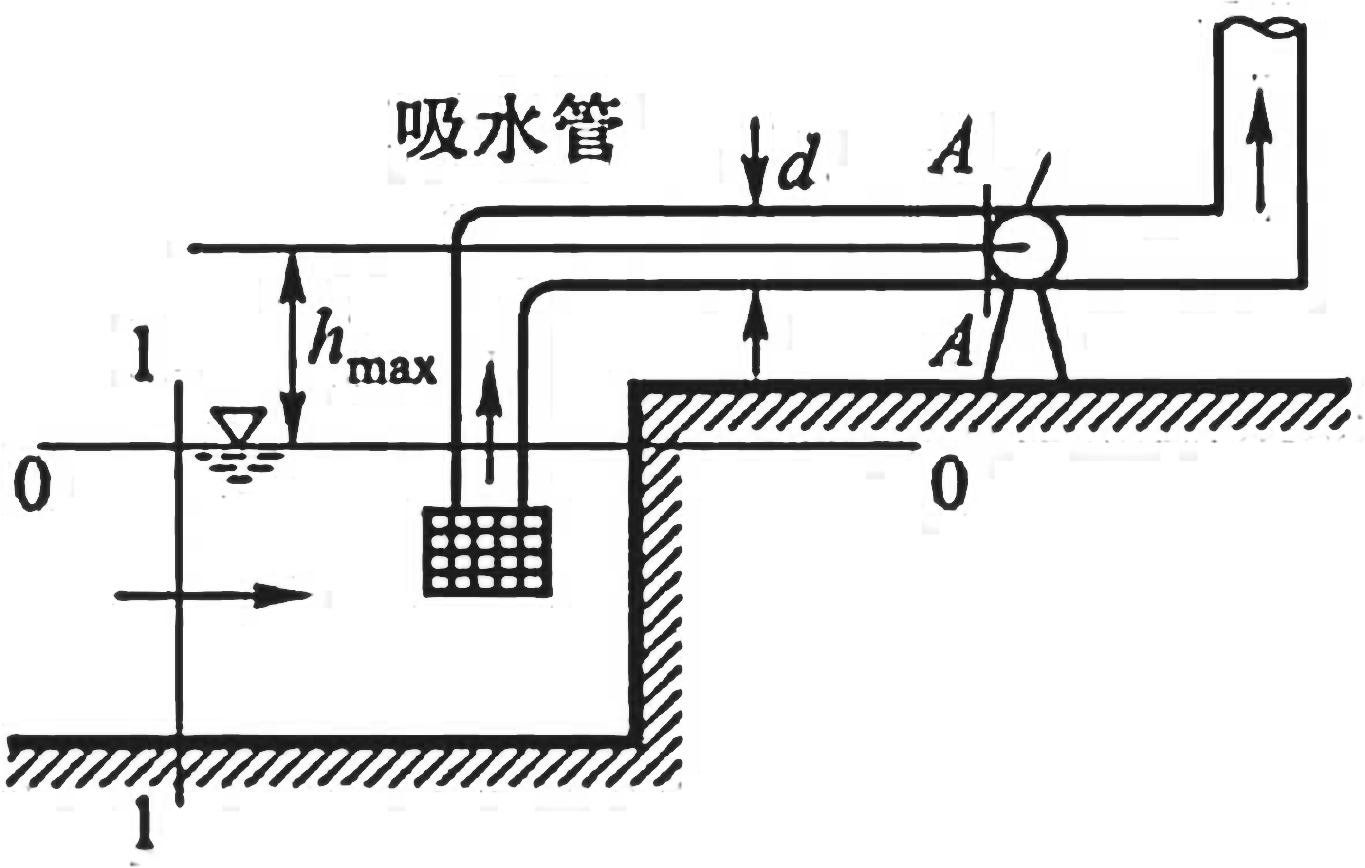
\includegraphics[width=\linewidth,height=0.45\textheight,keepaspectratio]{slides_assets/fluid_deck04/pump.png}\\
      {\scriptsize 图：源讲义原图}
  \end{columns}
\end{frame}

\begin{frame}{算例 F-3：文丘里管流量计（总流版）}
  水平管道 $D_1=200\,\mathrm{mm}$，喉部 $D_2=100\,\mathrm{mm}$；同液体压差计读数 $\Delta h=0.50\,\mathrm m$。取 $\alpha=1$ 且忽略损失。
  \begin{columns}[T]
    \column{0.63\textwidth}
      \footnotesize
      \[
        A_1=\pi(0.1)^2=0.03142\,\mathrm{m^2},\quad
        A_2=\pi(0.05)^2=0.007854\,\mathrm{m^2}.
      \]
      \[
        A_1v_1=A_2v_2,\qquad v_2=\frac{A_1}{A_2}v_1=4v_1.
      \]
      \[
        \frac{p_1-p_2}{\rho g}
        =
        \frac{v_2^2-v_1^2}{2g}
        =
        \frac{15v_1^2}{2g}.
      \]
      \[
        v_1=\sqrt{\frac{2g\Delta h}{15}}
        =
        \sqrt{\frac{2\times9.81\times0.50}{15}}
        =
        \sqrt{0.654}=0.809\,\mathrm{m/s}.
      \]
      \[
        Q=A_1v_1=0.03142\times0.809
        =0.02542\,\mathrm{m^3/s}\approx25.4\,\mathrm{L/s}.
      \]
    \column{0.37\textwidth}
      \centering
      \begin{tikzpicture}[scale=0.62,>={Stealth[length=5pt]}]
        \draw[fill=TLprimaryTint,draw=TLprimary,thick] (-2.4,0.65)--(-0.55,0.32)--(0.45,0.32)--(2.35,0.65)--(2.35,-0.65)--(0.45,-0.32)--(-0.55,-0.32)--(-2.4,-0.65)--cycle;
        \draw[->,TLaccent,thick] (-2.1,0)--(-1.2,0) node[midway,above] {$v_1$};
        \draw[->,TLaccent,thick] (-0.1,0)--(0.95,0) node[midway,above] {$v_2$};
        \draw[TLprimaryDark,thick] (-1.45,-0.65)--(-1.45,-1.45)--(0.05,-1.45)--(0.05,-0.32);
        \draw[TLaccent,thick] (-1.05,-1.45)--(-1.05,-0.95)--(-0.35,-0.95)--(-0.35,-1.45);
        \draw[<->,TLaccent,thick] (-0.25,-1.45)--(-0.25,-0.95) node[midway,right] {$\Delta h$};
        \node[TLinkSoft,align=center,text width=4.2cm] at (0,-2.05) {压差来自喉部速度水头增大};
      \end{tikzpicture}
  \end{columns}
\end{frame}

\TLsection{常见误区}

\begin{frame}{常见误区：水头线不是“越低越会流”}
  \TLwarnblock{误区 1：水总从高处或压强大处流}{
    错。恒定总流按\TLterm{机械能水头}从大到小流动；单看位置水头 $z$ 或压强水头 $p/(\rho g)$ 都不够。虹吸管可把水先带到高处，文丘里管中窄处压强较低但流速较大。
  }
  \[
    H=z+\frac{p}{\rho g}+\frac{\alpha v^2}{2g}
    =H_p+\frac{\alpha v^2}{2g},\qquad
    H_p=z+\frac{p}{\rho g}. \tag{T10}
  \]
  \TLwarnblock{误区 2：测压管水头线必须沿程下降}{
    错。总水头线在无泵无机组输入时沿程下降；测压管水头线 $H_p$ 可升、可降、也可不变。物理上 $H_p$ 不能高于同断面的总水头线，因为二者差值是速度水头。
  }
  \TLtakeaway{判断流动方向看总水头 $H$；判断压强变化看测压管水头 $H_p$，两条线回答的问题不同。}
\end{frame}

\begin{frame}{常见误区：把动量方程和能量方程混用}
  \TLwarnblock{误区 3：能量方程也能按坐标分解}{
    错。动量方程是矢量方程，可投影到 $x,y,z$ 三个方向；能量方程是标量方程，只比较单位重量机械能，不能拆成“水平能量”和“竖直能量”。
  }
  \[
    \sum \vc F=\rho Q(\beta_2\vc v_2-\beta_1\vc v_1),
    \qquad
    H_1=H_2+h_w. \tag{T11}
  \]
  \TLwarnblock{误区 4：动量流量就是平均流速乘以质量流量}{
    不严格。平均速度写法忽略了断面速度分布，严格总流动量通量要乘动量修正系数 $\beta$。只有速度分布均匀或工程近似取 $\beta\approx1$ 时，才可近似写成 $\dot m\,\vc v$。
  }
  \TLtakeaway{求力时用动量方程并画坐标；求流速、压强、水头时用能量方程并检查损失项。}
\end{frame}

\TLsection{练习题}

\begin{frame}{练习 H1（习题 \#23）$\star$：串联三段管}
  \TLinfoblock{题目}{
    三段圆管串联，直径分别为 $d_1=100\,\mathrm{mm}$、$d_2=50\,\mathrm{mm}$、$d_3=25\,\mathrm{mm}$。已知第三段平均流速 $v_3=10\,\mathrm{m/s}$，求 $v_1$、$v_2$ 与体积流量 $Q$。
  }
  \[
    A_i=\frac{\pi d_i^2}{4},\qquad Q=A_1v_1=A_2v_2=A_3v_3. \tag{T12}
  \]
  \begin{itemize}
    \item 提示 1：液体恒定串联流动直接使用不可压缩连续性方程 (T2)。
    \item 提示 2：先用直径平方比求 $A_3/A_1$ 和 $A_3/A_2$，不必先算出每个面积。
    \item 提示 3：流量最后用 $Q=A_3v_3$，单位要换成 $\mathrm{m^3/s}$。
  \end{itemize}
  \TLtakeaway{本题只考一个核心动作：同一串联管路中 $Q$ 处处相同。}
\end{frame}

\begin{frame}{练习 H2（习题 \#32）$\star\star$：阀门开闭求流量}
  \TLinfoblock{题目}{
    水管直径 $d=50\,\mathrm{mm}$。末端阀门关闭时压力表读数为 $21\,\mathrm{kPa}$，阀门开启后读数降为 $5.5\,\mathrm{kPa}$。不计水头损失，求通过流量 $Q$。
  }
  {\centering
  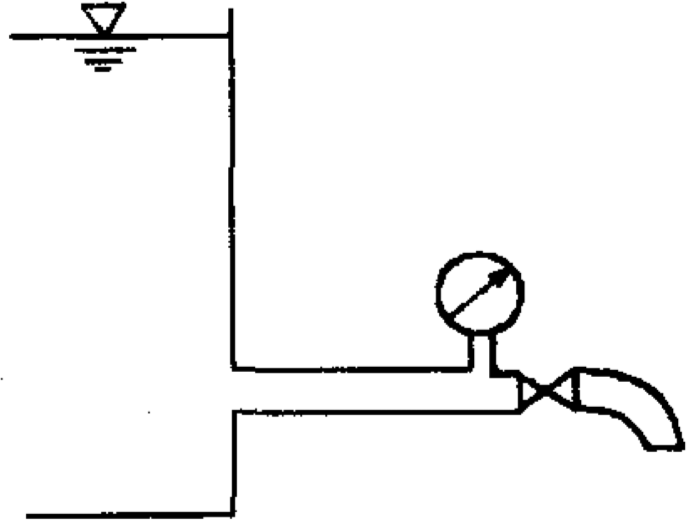
\includegraphics[width=0.5\textwidth,height=0.04\textheight,keepaspectratio]{slides_assets/fluid_deck04/ex-valve.png}\\[-0.3ex]
  {\scriptsize 图：源讲义原图}\par\vspace{-1.2\baselineskip}}
  \[
    \Delta p=p_{\text{关}}-p_{\text{开}},\qquad
    \frac{\Delta p}{\rho g}=\frac{v^2}{2g}. \tag{T13}
  \]
  \begin{itemize}
    \item 提示 1：关阀读数表示该点静止时可用的压强水头。
    \item 提示 2：开阀后压强下降的部分转化为速度水头。
    \item 提示 3：先求 $v=\sqrt{2\Delta p/\rho}$，再用 $Q=(\pi d^2/4)v$。
  \end{itemize}
  \TLtakeaway{本题练习伯努利方程中“压强水头差 $\leftrightarrow$ 速度水头”的转换。}
\end{frame}

\begin{frame}{练习 H3（习题 \#41）$\star\star$：变径管压差计}
  \TLinfoblock{题目}{
    水平变径管中水流量 $Q=0.1\,\mathrm{m^3/s}$，管径 $d_1=300\,\mathrm{mm}$、$d_2=100\,\mathrm{mm}$。两接压点在同一水平面，不计损失，求 U 形水银压差计读数 $h$。
  }
  {\centering
  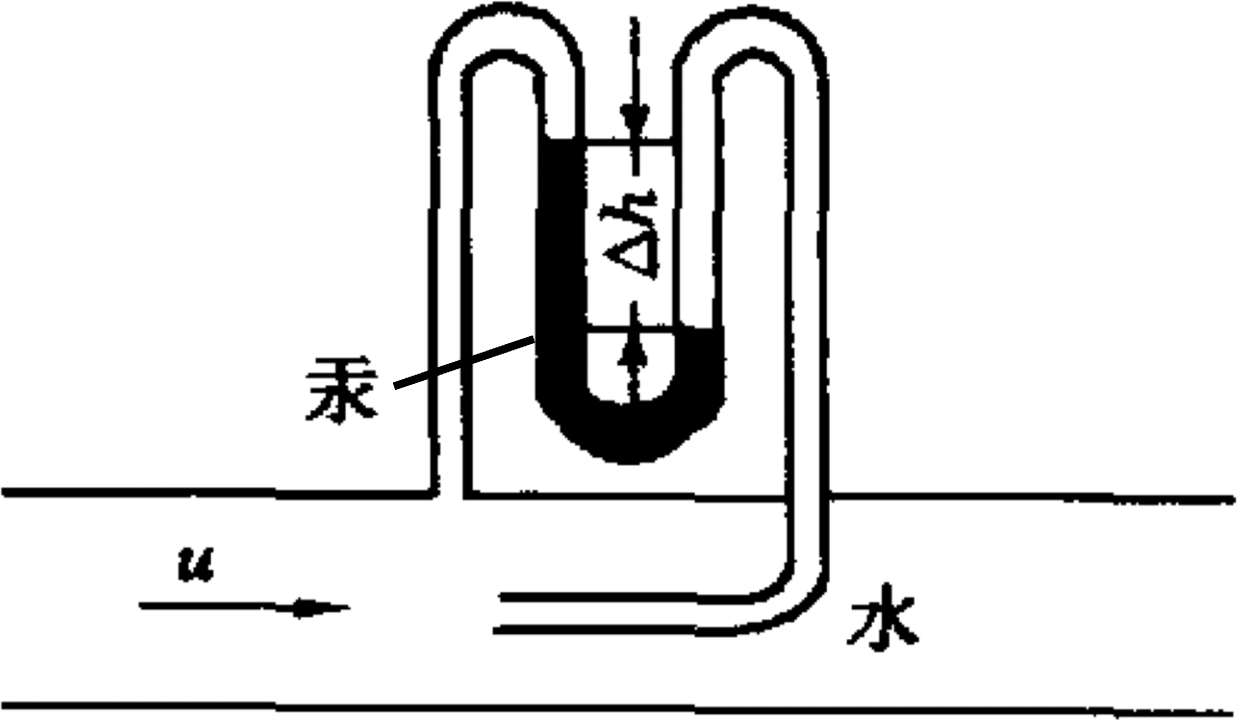
\includegraphics[width=0.5\textwidth,height=0.04\textheight,keepaspectratio]{slides_assets/fluid_deck04/ex-umanometer.png}\\[-0.3ex]
  {\scriptsize 图：源讲义原图}\par\vspace{-1.2\baselineskip}}
  \[
    \Delta p=p_1-p_2
    =\rho_w\frac{v_2^2-v_1^2}{2},
    \qquad
    \Delta p=(\rho_{\mathrm{Hg}}-\rho_w)gh. \tag{T14}
  \]
  \begin{itemize}
    \item 提示 1：先用 (T12) 的面积公式求 $A_1,A_2$，再由 $v_i=Q/A_i$ 求速度。
    \item 提示 2：两接压点同高，所以伯努利方程中 $z_1=z_2$。
    \item 提示 3：压差计内是水银，换算压差时用密度差 $\rho_{\mathrm{Hg}}-\rho_w$。
  \end{itemize}
  \TLtakeaway{本题把连续性、伯努利和压差计读数三件事串在一起。}
\end{frame}

\begin{frame}{练习 H4（习题 \#43）$\star\star\star$：虹吸管真空校核}
  \TLinfoblock{题目}{
    虹吸管直径 $d=0.2\,\mathrm m$，最高点 $B$ 高出上游水面 $h_1=2\,\mathrm m$，出口低于上游水面 $h_2=4\,\mathrm m$。取 $\alpha=1$ 且不计损失，求流量 $Q$，并校核 $B$ 点真空度是否超过 $7\,\mathrm m$ 水柱。
  }
  {\centering
  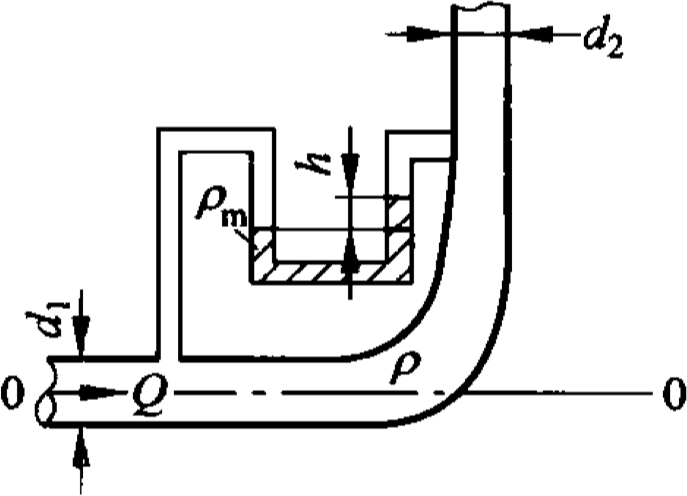
\includegraphics[width=0.5\textwidth,height=0.04\textheight,keepaspectratio]{slides_assets/fluid_deck04/ex-siphon.png}\\[-0.3ex]
  {\scriptsize 图：源讲义原图}\par\vspace{-1.2\baselineskip}}
  \[
    h_1+h_2=\frac{v^2}{2g},
    \qquad
    H_{\mathrm{vac},B}=h_1+\frac{v^2}{2g}. \tag{T15}
  \]
  \begin{itemize}
    \item 提示 1：从上游自由水面到出口断面列总流能量方程。
    \item 提示 2：自由水面与出口都通大气，相对压强项均为零。
    \item 提示 3：真空校核必须在最高点 $B$ 做；比较的是 $H_{\mathrm{vac},B}$ 与允许值 $7\,\mathrm m$。
  \end{itemize}
  \TLtakeaway{虹吸题不能只求流量；最高点真空度可能使设计不合格。}
\end{frame}

\begin{frame}{练习 H5（习题 \#44）$\star\star\star$：倒虹吸管流量}
  \TLinfoblock{题目}{
    倒虹吸管直径 $d=0.1\,\mathrm m$，上下游水面高度差 $H=3\,\mathrm m$。总水头损失等于管中一个速度水头，即 $h_L=v^2/(2g)$。求通过流量 $Q$。
  }
  {\centering
  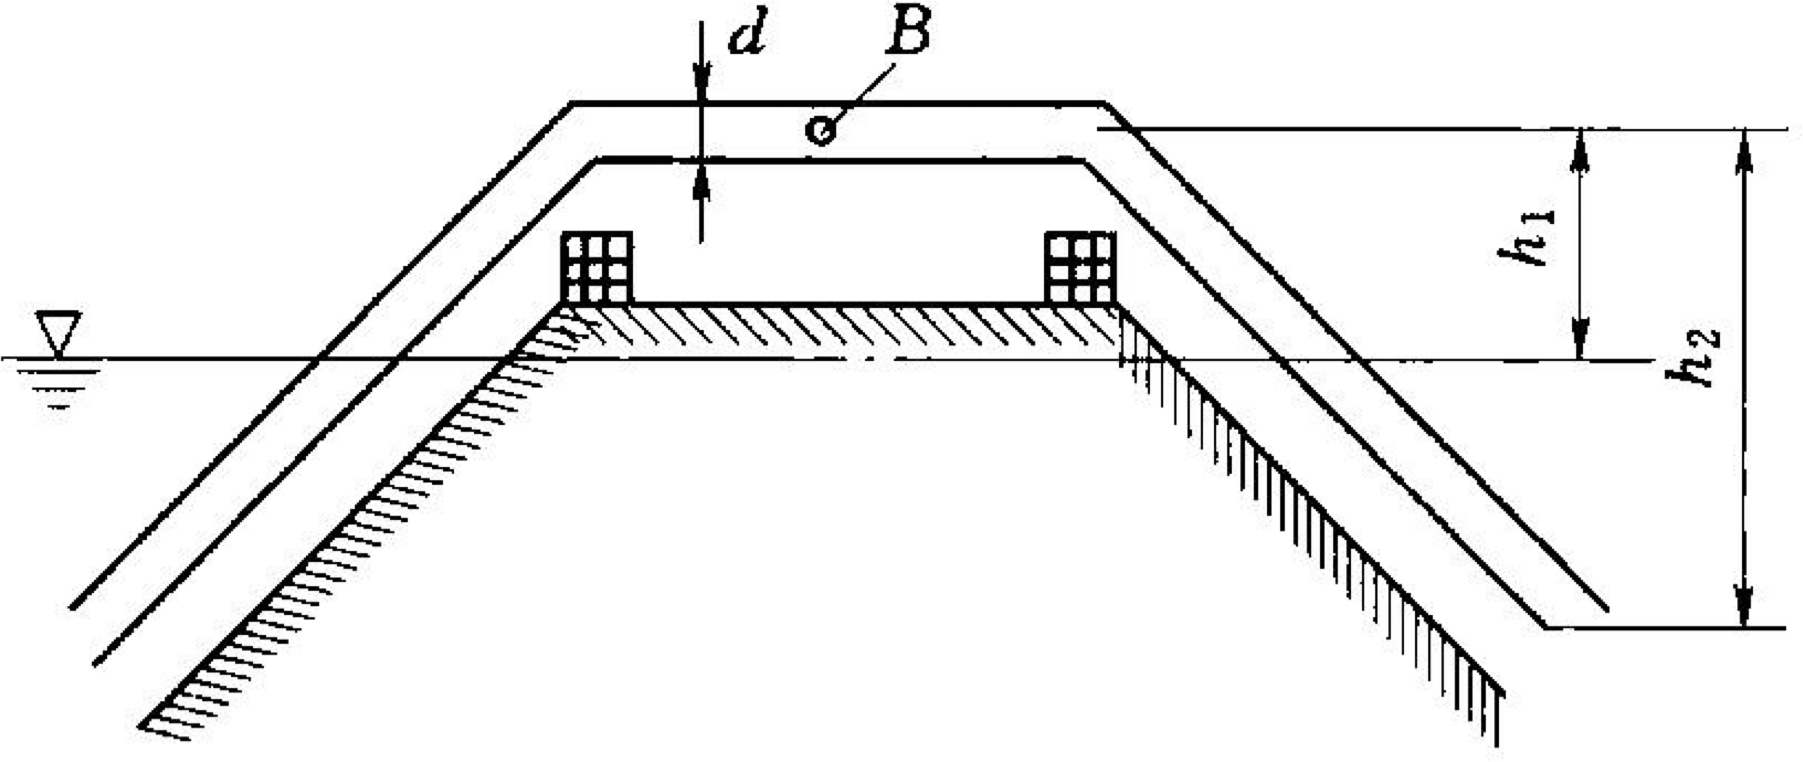
\includegraphics[width=0.5\textwidth,height=0.04\textheight,keepaspectratio]{slides_assets/fluid_deck04/ex-inv-siphon.png}\\[-0.3ex]
  {\scriptsize 图：源讲义原图}\par\vspace{-1.2\baselineskip}}
  \[
    H=\frac{v^2}{2g}+h_L
    =\frac{v^2}{2g}+\frac{v^2}{2g}
    =\frac{v^2}{g}. \tag{T16}
  \]
  \begin{itemize}
    \item 提示 1：两个自由水面均取相对压强为零，水面速度近似为零。
    \item 提示 2：本题损失不是零，而是一个速度水头。
    \item 提示 3：由 $v=\sqrt{gH}$ 求速度，再用 $Q=(\pi d^2/4)v$ 求流量。
  \end{itemize}
  \TLtakeaway{倒虹吸题的关键是把可用水头分成出口速度水头和损失水头两部分。}
\end{frame}

\TLsection{延伸与文献注记}

\begin{frame}{源讲义 §4.4：本 deck 的位置}
  本 deck 对应源讲义第四章 §4.4“一元恒定流基本原理”，把源讲义中的总流方程、经典仪器和计算题改写成可独立复算的自学材料。
  \begin{center}
  \vspace{4pt}
  \footnotesize
  \setlength{\tabcolsep}{4pt}
  \begin{tabular}{@{}lll@{}}
    \toprule
    源讲义段落 & 本 deck 主线 & 自学补足 \\
    \midrule
    4.4.1 & 连续性方程 & 从控制体通量推到 $Q_1=Q_2$ \\
    4.4.2 & 动量方程 & 写清矢量、分量和受力正负号 \\
    4.4.3 & 元流伯努利 & 解释三种水头和成立条件 \\
    4.4.4 & 总流能量 & 加入 $\alpha$、水头损失和水头线 \\
    习题 23--44 & 计算训练 & 题面提示与附录逐步全解 \\
    \bottomrule
  \end{tabular}
  \end{center}
  \TLtakeaway{源讲义给出标准结论；本 deck 的任务是把每个结论的使用条件和计算步骤写到页内。}
\end{frame}

\begin{frame}{人物线索：伯努利、皮托与文丘里}
  这一节的许多仪器名来自十八世纪流体力学的三条线索：能量、测速和收缩压差。
  \begin{center}
  \vspace{4pt}
  \footnotesize
  \setlength{\tabcolsep}{3pt}
  \begin{tabular}{@{}lll@{}}
    \toprule
    人物 & 年代 & 与本 deck 的关系 \\
    \midrule
    Daniel Bernoulli & 1700--1782 & 伯努利方程，把压强、速度和高度联系为机械能 \\
    Johann Bernoulli & 1667--1748 & Daniel 之父，推动早期流体力学和变分思想 \\
    Henri Pitot & 1695--1771 & 皮托管，用滞止压和静压差测速度 \\
    Giovanni Venturi & 1746--1822 & 文丘里效应，用收缩段压强降低测流量 \\
    \bottomrule
  \end{tabular}
  \end{center}
  \[
    \text{能量守恒}
    \longrightarrow
    \text{速度--压强互换}
    \longrightarrow
    \text{测速与流量计}. \tag{T17}
  \]
  \TLtakeaway{这些名字不只是历史标签；它们分别对应本章最常用的方程和测量装置。}
\end{frame}

\begin{frame}{工程应用：速度水头与压强水头互换}
  伯努利思想最常见的工程用法，是把速度增大与压强降低联系起来，但每次使用都要先检查是否可近似忽略损失。
  \begin{center}
  \vspace{4pt}
  \footnotesize
  \setlength{\tabcolsep}{4pt}
  \begin{tabular}{@{}lll@{}}
    \toprule
    场景 & 直觉图像 & 需要保留的限制 \\
    \midrule
    机翼升力定性 & 上表面流速较大，压强较低 & 真实升力还依赖粘性和环量 \\
    化油器 & 喉部低压吸入燃油 & 需考虑局部损失和雾化 \\
    喷射泵 & 高速射流形成负压抽吸 & 能量损失通常不可忽略 \\
    水电站引水管 & 水头差转化为速度和机组能量 & 需计沿程、局部和机组项 \\
    \bottomrule
  \end{tabular}
  \end{center}
  \[
    \Delta\left(\frac{p}{\rho g}\right)
    \approx
    -\,\Delta\left(\frac{v^2}{2g}\right)
    \quad\text{只是在同高、无损、}\alpha=1\text{ 的近似下成立。}
  \]
  \TLtakeaway{“高速等于低压”是有条件的判断，不是可以脱离断面、损失和高度的口号。}
\end{frame}

\begin{frame}{修正系数与后续章节}
  $\alpha$ 和 $\beta$ 记录断面速度分布的不均匀性。本 deck 常取 $1$ 是为了先学会列方程；后续水头损失和管流章节会解释它们何时不能忽略。
  \begin{center}
  \vspace{4pt}
  \footnotesize
  \setlength{\tabcolsep}{4pt}
  \begin{tabular}{@{}lll@{}}
    \toprule
    流动类型 & 动能修正系数 $\alpha$ & 动量修正系数 $\beta$ \\
    \midrule
    均匀速度分布 & $1$ & $1$ \\
    圆管层流 & $2$ & $4/3$ \\
    圆管紊流工程近似 & $1.05$--$1.10$ & $1.02$--$1.05$ \\
    粗略估算 & 常取 $1$ & 常取 $1$ \\
    \bottomrule
  \end{tabular}
  \end{center}
  推荐路线：闻德荪《流体力学》和吴持恭《水力学》适合中文水力学习题，White, \emph{Fluid Mechanics} 适合工程流体力学视角。外部链接只作深化，本讲义本身完整。
  \TLtakeaway{本章先学“会列方程”；Deck 5/6 再处理速度分布、阻力和水头损失的来源。}
\end{frame}

\TLsection{术语速查}

\begin{frame}{术语速查（一）：总流与三大方程}
  \begin{center}
  \vspace{4pt}
  \footnotesize
  \setlength{\tabcolsep}{2.5pt}
  \begin{tabular}{@{}p{0.24\textwidth}p{0.30\textwidth}p{0.34\textwidth}@{}}
    \toprule
    中文术语 & English & Symbol/Eq \\
    \midrule
    总流 & total stream & 断面平均后的一维流动 \\
    过水断面 & flow cross-section & $A$ \\
    流量 & flow rate & $Q=vA$ \\
    流速 & mean velocity & $v=Q/A$ \\
    连续性方程 & continuity equation & (T2), (T3) \\
    能量方程 & energy equation & (T9), $H_1=H_2+h_w$ \\
    伯努利方程 & Bernoulli equation & (T8) \\
    动量方程 & momentum equation & (T6), (T11) \\
    动量修正系数 & momentum correction factor & $\beta$，见 (T5) \\
    动能修正系数 & kinetic-energy correction factor & $\alpha$ \\
    \bottomrule
  \end{tabular}
  \end{center}
  \TLtakeaway{第一组术语围绕“把三维流动压缩成总流方程”。}
\end{frame}

\begin{frame}{术语速查（二）：水头线、仪器与管路}
  \begin{center}
  \vspace{4pt}
  \footnotesize
  \setlength{\tabcolsep}{2.5pt}
  \begin{tabular}{@{}p{0.24\textwidth}p{0.30\textwidth}p{0.34\textwidth}@{}}
    \toprule
    中文术语 & English & Symbol/Eq \\
    \midrule
    水头 & head & 单位重量机械能的高度表示 \\
    测压管水头 & piezometric head & $H_p=z+p/(\rho g)$ \\
    位置水头 & elevation head & $z$ \\
    速度水头 & velocity head & $\alpha v^2/(2g)$ \\
    总水头线 & energy grade line & $H=z+p/(\rho g)+\alpha v^2/(2g)$ \\
    测压管水头线 & hydraulic grade line & $H_p$ 沿程曲线 \\
    水力坡度 & hydraulic gradient & $J=-\rd H/\rd s$ \\
    压差计 & differential manometer & (T14) \\
    虹吸管 & siphon & 最高点需校核真空度 \\
    倒虹吸 & inverted siphon & 管路下穿障碍后再上升 \\
    \bottomrule
  \end{tabular}
  \end{center}
  \TLtakeaway{第二组术语围绕“把能量方程画成水头线并用于测量”。}
\end{frame}

\appendix

\begin{frame}{附录解答·习题23（A1）}
  \footnotesize
  使用连续性方程 (T12)：串联管路中 $Q=A_1v_1=A_2v_2=A_3v_3$。先统一单位：
  \[
    d_1=0.100\,\mathrm m,\qquad d_2=0.050\,\mathrm m,\qquad d_3=0.025\,\mathrm m.
  \]
  由面积正比于直径平方：
  \[
    \frac{A_3}{A_1}=\left(\frac{d_3}{d_1}\right)^2
    =\left(\frac{0.025}{0.100}\right)^2
    =(0.25)^2=0.0625.
  \]
  \[
    v_1=\frac{A_3}{A_1}v_3=0.0625\times10=0.625\,\mathrm{m/s}.
  \]
  \[
    \frac{A_3}{A_2}=\left(\frac{0.025}{0.050}\right)^2
    =(0.5)^2=0.25,\qquad
    v_2=0.25\times10=2.5\,\mathrm{m/s}.
  \]
  \[
    A_3=\frac{\pi}{4}(0.025)^2=4.9087\times10^{-4}\,\mathrm{m^2},\quad
    Q=A_3v_3=4.9087\times10^{-4}\times10=4.9087\times10^{-3}\,\mathrm{m^3/s}.
  \]
  \[
    \boxed{v_1=0.625\,\mathrm{m/s},\quad v_2=2.5\,\mathrm{m/s},\quad Q\approx4.91\times10^{-3}\,\mathrm{m^3/s}.}
  \]
\end{frame}

\begin{frame}{附录解答·习题32（A2）}
  \footnotesize
  使用压强水头差转速度水头的能量关系 (T13)。压力表读数差为
  \[
    \Delta p=p_{\text{关}}-p_{\text{开}}
    =21\,\mathrm{kPa}-5.5\,\mathrm{kPa}
    =15.5\,\mathrm{kPa}
    =15500\,\mathrm{Pa}.
  \]
  由 (T13) 得
  \[
    \frac{\Delta p}{\rho g}=\frac{v^2}{2g}
    \quad\Longrightarrow\quad
    v=\sqrt{\frac{2\Delta p}{\rho}}.
  \]
  \[
    v=\sqrt{\frac{2\times15500}{1000}}
    =\sqrt{31}
    =5.568\,\mathrm{m/s}.
  \]
  管道面积为
  \[
    A=\frac{\pi}{4}d^2
    =\frac{\pi}{4}(0.050)^2
    =\frac{\pi}{4}\times0.0025
    =1.9635\times10^{-3}\,\mathrm{m^2}.
  \]
  \[
    Q=Av=1.9635\times10^{-3}\times5.568
    =1.0932\times10^{-2}\,\mathrm{m^3/s}.
  \]
  \[
    \boxed{v\approx5.57\,\mathrm{m/s},\qquad Q\approx1.094\times10^{-2}\,\mathrm{m^3/s}.}
  \]
\end{frame}

\begin{frame}{附录解答·习题41（A3）}
  \footnotesize
  使用连续性方程 (T12) 求速度，再用水平无损伯努利和压差计关系 (T14) 求 $h$。
  \begin{columns}[T]
    \column{0.49\textwidth}
      \[
        A_1=\frac{\pi}{4}(0.300)^2
        =7.0686\times10^{-2}\,\mathrm{m^2}.
      \]
      \[
        v_1=\frac{Q}{A_1}
        =\frac{0.1}{7.0686\times10^{-2}}
        =1.4147\,\mathrm{m/s}.
      \]
      \[
        A_2=\frac{\pi}{4}(0.100)^2
        =7.8540\times10^{-3}\,\mathrm{m^2}.
      \]
      \[
        v_2=\frac{0.1}{7.8540\times10^{-3}}
        =12.7324\,\mathrm{m/s}.
      \]
    \column{0.51\textwidth}
      \[
        v_1^2=(1.4147)^2=2.0014,\qquad
        v_2^2=(12.7324)^2=162.1139.
      \]
      \[
        \frac{v_2^2-v_1^2}{2}
        =\frac{162.1139-2.0014}{2}
        =80.0562\,\mathrm{m^2/s^2}.
      \]
      \[
        \Delta p=1000\times80.0562=80056\,\mathrm{Pa}.
      \]
      \[
        (\rho_{\mathrm{Hg}}-\rho_w)g=(13600-1000)\times9.81=123606\,\mathrm{N/m^3}.
      \]
  \end{columns}
  \[
    h=\frac{80056}{123606}=0.6477\,\mathrm m,
    \qquad
    \boxed{h\approx0.648\,\mathrm m.}
  \]
\end{frame}

\begin{frame}{附录解答·习题43（A4）}
  \footnotesize
  使用虹吸管能量关系 (T15)。从上游自由水面到出口断面列方程；两端均通大气，速度水头只保留管内速度。
  \[
    h_1+h_2=2+4=6\,\mathrm m.
  \]
  \[
    \frac{v^2}{2g}=6
    \quad\Longrightarrow\quad
    v=\sqrt{2g\times6}.
  \]
  \[
    v=\sqrt{2\times9.81\times6}
    =\sqrt{117.72}
    =10.8499\,\mathrm{m/s}.
  \]
  \[
    A=\frac{\pi}{4}d^2
    =\frac{\pi}{4}(0.2)^2
    =\frac{\pi}{4}\times0.04
    =3.1416\times10^{-2}\,\mathrm{m^2}.
  \]
  \[
    Q=Av=3.1416\times10^{-2}\times10.8499
    =0.3409\,\mathrm{m^3/s}.
  \]
  最高点 $B$ 的真空度由 (T15) 给出：
  \[
    H_{\mathrm{vac},B}=h_1+\frac{v^2}{2g}=2+6=8\,\mathrm m.
  \]
  \[
    \boxed{Q\approx0.341\,\mathrm{m^3/s},\qquad H_{\mathrm{vac},B}=8\,\mathrm m>7\,\mathrm m,\ \text{设计不合格。}}
  \]
\end{frame}

\begin{frame}{附录解答·习题44（A5）}
  \footnotesize
  使用倒虹吸能量关系 (T16)。两个自由水面均用相对压强，水面速度近似为零；题目给定总损失为一个速度水头。
  \[
    H=\frac{v^2}{2g}+h_L,
    \qquad
    h_L=\frac{v^2}{2g}.
  \]
  \[
    H=\frac{v^2}{2g}+\frac{v^2}{2g}
    =\frac{v^2}{g}.
  \]
  \[
    v^2=gH=9.81\times3=29.43.
  \]
  \[
    v=\sqrt{29.43}=5.4249\,\mathrm{m/s}.
  \]
  管道面积为
  \[
    A=\frac{\pi}{4}d^2
    =\frac{\pi}{4}(0.1)^2
    =\frac{\pi}{4}\times0.01
    =7.8540\times10^{-3}\,\mathrm{m^2}.
  \]
  \[
    Q=Av
    =7.8540\times10^{-3}\times5.4249
    =4.2607\times10^{-2}\,\mathrm{m^3/s}.
  \]
  \[
    \boxed{v\approx5.42\,\mathrm{m/s},\qquad Q\approx4.26\times10^{-2}\,\mathrm{m^3/s}.}
  \]
\end{frame}

\end{document}
